\chapter{几何 Satake}\label{ch:11}

\begin{keytakeaways}
本章讲述几何 Satake 对应：仿射 Grassmann 流形$\Gr_G=G(K)/G(\cO)$在$LG_+$-等变层下的范畴$\sph$，作为对称幺半范畴，等价于 Langlands 对偶群$G^{\vee}$的表示范畴。技术路线是：先观察到$\Gr_G$的$LG_+$-轨道由余权格$\Lambda$模 Weyl 群标号，再借由抛物限制把$\Gr_G$上的层拉回到$\Gr_T\simeq\Lambda$上的层，从而用 Fourier 级数（Tannakian 重构）读出$G^{\vee}$；几何 Satake 定理正是这一重构的严格化。由此，$\sph$以 Hecke 算子的形式作用在$\Shv(\Bun_G(C))$上，其谱分解给出几何 Langlands 纲领的 Hecke 特征层，并在物理上对应规范理论$A_G$与 4 维 B-模型$B_{G^{\vee}}$的电磁对偶。
\end{keytakeaways}

\section{总体思想}\label{sec:11-1}

\begin{sectionkey}
本节回顾贯穿全书的“群胚作用”图景：一个带$K$-作用的空间$X$给出群胚$X/K\rightrightarrows \mathrm{pt}/K$，并给出 Hecke 对应；平衡积$\times^K$是把$G/K$丛化到$X/K$上的标准工具。
\end{sectionkey}

\begin{flushright}\small 第 26 讲；2021 年 4 月 29 日\end{flushright}

回顾一般图景：当给定$X\supset K$（即$K$作用于$X$）时，我们有一个群胚作用：
\begin{equation}\tag{11.1}
\begin{array}{ccc}
X/K & \quad\circlearrowleft\quad & K\backslash G/K\\[2pt]
 & \searrow\ \swarrow & \\[2pt]
 & \mathrm{pt}/K &
\end{array}
\end{equation}
或者等价地，我们有一个由 Hecke 给出的对应：
\begin{equation}\tag{11.2}
\begin{array}{ccc}
 & \operatorname{Hecke} & \\
 \swarrow & & \searrow\\
 X/K & & X/K
\end{array}
\end{equation}
其中$\operatorname{Hecke}$是$X/K$上由主$K$-丛$X\to X/K$诱导的$G/K$-丛，也就是说，我们把$G/K$看成带$K$-作用的空间，于是有：
\begin{equation}\tag{11.3}
\operatorname{Hecke}=X\times^{K}G/K,
\end{equation}
其中$\times^{K}$表示\term{平衡积}{balanced product}，即我们已经对$X$上$K$的右作用和$G/K$上$K$的左作用作了商。

% [Tutor Note: 原文记号$X\supset K$是“$K$作用在$X$上”的简写，并非包含关系；平衡积$X\times^KG/K$的严格含义是$(X\times G/K)/K$，其中$k\cdot(x,gK)=(xk^{-1},kgK)$。这一约定在 (11.14) 的$LG_+$-丛中反复使用，读者若不熟悉伴随丛的构造，可对照 [Bor91] 或任何主丛教材。]

\section{仿射 Grassmann 流形}\label{sec:11-2}

\begin{sectionkey}
本节定义\term{仿射 Grassmann 流形}{affine Grassmannian} $\Gr_G=G(K)/G(\cO)=LG/LG_+$，把它实现为圆盘上平凡$G$-丛在一点处的修正，并说明其上的$LG_+$-轨道等价于分数维 Hecke 对应的核；最后（11.2.1–11.2.2）讨论它的同伦型$\Omega G_c$与 Bialynicki-Birula 胞腔分解。
\end{sectionkey}

对$x\in C$，我们将构造$\operatorname{Hecke}$的一个版本，称为$\operatorname{Hecke}_x$：
\begin{equation}\tag{11.4}
\begin{array}{ccc}
 & \operatorname{Hecke}_x & \\
 \swarrow & & \searrow\\
 \Bun_G(C) & & \Bun_G(C)
\end{array}
\end{equation}

这是一个纤维化，其纤维由仿射 Grassmann 流形给出：
\begin{align}
\Gr_G&:=G(K_x)/G(\cO_x)\tag{11.5}\\
&=LG/LG_+.\tag{11.6}
\end{align}
我们可以这样看：
\begin{equation}\tag{11.7}
G(K_x)=LG=\operatorname{Map}(D^{*},G),
\end{equation}
而在其中我们有：
\begin{equation}\tag{11.8}
G(K_x)\supset G(\cO_x)=LG_+=\operatorname{Map}(D,G).
\end{equation}
对任意曲线$C$，$\Gr$可以写成：
\begin{align}
\Gr_G&=LG/LG_+\tag{11.9}\\
&=\{\text{$C$上的$G$-丛，且在 }C\setminus x\text{ 上平凡}\}\tag{11.10}\\
&=\{\text{$D$上的$G$-丛，且在 }D\setminus x\text{ 上平凡}\},\tag{11.11}
\end{align}
即它由$D$上平凡丛在点$x$处的修正组成。

我们可以把$\operatorname{Hecke}_x$明确写成三元组的集合：
\begin{align}
\operatorname{Hecke}_x&=\Bigl\{P_1,P_2\in\Bun_G(X),\ P_1|_{C\setminus x}\xrightarrow{\ \sim\ }P_2|_{C\setminus x}\Bigr\}\tag{11.12}\\
&=\Bigl\{P_1,\ P_2|_{D},\ P_1|_{D^{*}}\xrightarrow{\ \sim\ }P_2|_{D^{*}}\Bigr\}.\tag{11.13}
\end{align}
上面的描述清楚地表明我们有两个到$\Bun_G(C)$的映射（一个把三元组送到$P_1$，另一个送到$P_2$），但下面的描述告诉我们，$\operatorname{Hecke}$与$\Bun_G$上的主$LG_+$-丛相关联，该丛由$\Bun_G(C,x)$（在$D_x$上有平凡化的$G$-丛构成的空间）给出。也就是说：
\begin{equation}\tag{11.14}
\operatorname{Hecke}_X=\Bun_G(C,x)\times^{LG_+}\Gr.
\end{equation}
也就是说，我们从$P\in\Bun_G$出发并在$D$上平凡化，于是得到$P$连同平凡化这一对，即$\Bun_G(C,x)$中的对象。然后我们修正$D$上的平凡丛，以在$\Bun_G(C,x)\times\Gr$中得到$P$和$P'$，接着对$G(\cO)=LG_+$取商。

于是$\operatorname{Hecke}_x$以两种方式成为$\Bun_G$上的扭$\Gr$-丛：
\begin{equation}\tag{11.15}
\begin{array}{ccccc}
 & & \operatorname{Hecke}_x & & \\
 & \swarrow & & \searrow & \\
\Bun_G & & & & \Bun_G\\
 & \searrow & & \swarrow & \\
 & & \Gr & &
\end{array}
\end{equation}
例如通过映到$P$或映到$P'$。

这有什么用处？$\operatorname{Hecke}$是一个群胚，因此我们可以尝试用它作用在$\Bun_G$上。确定$\operatorname{Hecke}$中的点并不容易，但我们可以挑出轨道。局部地，一旦选定平凡化，它看起来就像$\Gr\times\Bun_G$。若改变平凡化，则这一识别差一个左作用$LG_+\circlearrowright\Gr$。这其实只是伴随丛的一般事实：$\Gr$上任何$LG_+$-不变的对象在整空间$\operatorname{Hecke}_x$上都有意义。例如若取$\Gr$中任何$LG_+$-轨道$O$，即$O$对应一个陪集$LG_+\backslash LG/LG$，则这给出$\Bun_G$与自身之间的一个对应：
\begin{equation}\tag{11.16}
\begin{array}{ccc}
 & O & \\
 \swarrow & & \searrow\\
 \Bun_G & & \Bun_G
\end{array}
\end{equation}
因此，给定这一个对象$\operatorname{Hecke}_x$，我们应当把它看成给出许多不同的对应，以$\Gr$中的轨道为标号。

\begin{srcex}{71}
回忆在例 70 中我们取$G=GL_n$，并对任意满足$0\le k\le n$的整数$k$得到一个对应：
\begin{equation}\tag{11.17}
\begin{array}{ccccc}
 & & \operatorname{Hecke}_x^{k} & & \\
 & \swarrow & & \searrow & \\
\Bun_n(C) & & & & \Bun_n(C)\\
 & \searrow & & \swarrow & \\
 & & \Gr_k^n & &
\end{array}
\end{equation}
\end{srcex}
这个$\operatorname{Hecke}_x^{k}$就是来自$\Gr$中轨道的对应之一例。事实上，$GL_n(\cO)=L(GL_n)_+$在
\begin{equation}\tag{11.18}
\Gr_{GL_n}=GL_n(K)/GL_n(\cO)
\end{equation}
上的闭轨道与整数$0\le k\le n$一一对应，且同构于通常的 Grassmann 流形$\Gr_k^n$。具体地，$\Gr_{GL_n}$由圆盘$D$上秩为$n$的向量丛$V$连同$D^{*}$上的平凡化组成。我们可以非常具体地写出如下。考虑$V$在圆盘上的正则截面$V(D)$。它位于去心圆盘上的截面空间之内，而后者已被平凡化：
\begin{equation}\tag{11.19}
V(D)\subset V(D^{*})\cong K^{n},
\end{equation}
所以这是$K^{n}$的子空间，即$n$份 Laurent 级数。事实上，这不仅是子空间，还是$K^{n}$的$\cO$-子模。若把参数取逆，我们得到：
\begin{equation}\tag{11.20}
V(D)\otimes_{\cO}K\simeq K^{n}.
\end{equation}
换言之，仿射 Grassmann 流形就是$K^{n}$内所有$\cO$-格的集合。

我们可以用某个$N$来界定极点的阶，于是发现子空间$V(D)$被夹在：
\begin{equation}\tag{11.21}
t^{-N}\cO^{n}\subset V(D)\subset t^{N}\cO^{n}\subset K^{n}.
\end{equation}
这个夹层两端的商是有限维向量空间，因此$V(D)$给出其中一个子空间。它还对坐标乘法封闭。无论如何，它是有限维 Grassmann 流形的一个闭子簇。于是我们得到$\Gr_n$的描述
\begin{equation}\tag{11.22}
\Gr_n=\bigcup_{N}\{\text{射影簇}\}.
\end{equation}
即$\Gr_n$是 ind-真（ind-proper）ind-概形。对其他群，我们可以通过选取到$GL_n$的忠实表示，把相应的$\Gr_G$嵌入$\Gr_n$。对$N=1$，我们可以看到有限维的$\Gr_k^n$作为轨道位于其中。

所以思路是：我们研究$\Gr$，但只想研究在$G(\cO)$作用下不变的几何。任何这样的几何在$\Bun_G$上都有意义。例如我们可以考虑不变层$\Shv^{G(\cO)}(\Gr)$，然后它映到$\Shv(\operatorname{Hecke}_x)$。因此，通过$\operatorname{Hecke}_x$的群胚作用，我们得到$\Bun_G$上的积分核，即有映射：
\begin{equation}\tag{11.23}
\Shv^{G(\cO)}(\Gr)\longrightarrow\Shv(\operatorname{Hecke}_x)\longrightarrow\End\bigl(\Shv(\Bun_G)\bigr).
\end{equation}
再次：
\begin{equation}\tag{11.24}
\Shv^{G(\cO)}(\Gr)=\Shv\bigl(G(\cO)\backslash G(K)/G(\cO)\bigr)=:\sph.
\end{equation}
于是轨道$O$通过考察$O$上常值层在这两个映射下的像给出一个算子。在物理图景中，我们在某点$x\in C$和某时刻$t\in I$插入$O$：
\diageq{11.25}{0.14\textwidth}{p182_d1.png}
结合律来自$\{x\}\times I$上三点构型的结合性。交换律则是因为，给定放置算子的两个这样的点，我们有足够的维数让这些点交换位置。现在我们要从物理中提炼这一想法，以看出这些 Hecke 算子是交换的。关键在于$\Gr$带有某种额外的代数结构，其形式并不十分常见，来源于移动点$x\in C$。

% [Tutor Note: (11.14) 原文写作$\operatorname{Hecke}_X$，而其余各处均为$\operatorname{Hecke}_x$，是记号笔误（$x$为曲线上一点，$X$为曲线/概形），译文保留原式并在此指出。(11.22) 中的并集应理解为$\mathrm{colim}_N$，故只能说$\Gr_n$是 ind-真 ind-概形而非真概形。]

\subsection{$\Gr$的同伦型}\label{sec:11-2-1}

回忆对$G=GL_1$有$\Gr_1=\Z$。我们的 Fourier 级数描述正来源于此。所以$\Gr$是$\Z$的某种推广。按定义，$\Gr$由$\bA^{1}$上的$G$-丛连同$\bA^{1}\setminus 0$上的平凡化组成。若只考虑$\Gr$的同伦型，我们可以把它想成：
\begin{equation}\tag{11.26}
\Gr=\{\text{$\R^{2}$上的$G$-丛}+\text{$\R^{2}\setminus D_0$上的平凡化}\}.
\end{equation}
我们还可以再往前一步，取：
\begin{align}
\Gr&\simeq\{\text{$\R^{2}$上的$G_c$-丛}+\text{$\R^{2}\setminus D_0$上的平凡化}\}\tag{11.27}\\
&\simeq\operatorname{Map}\bigl((\R^{2},\R^{2}\setminus D);(BG,*)\bigr)\tag{11.28}\\
&\simeq\Omega^{2}BG\tag{11.29}\\
&\simeq\Omega G\tag{11.30}\\
&\simeq\Omega G_c,\tag{11.31}
\end{align}
其中$D_0$是围绕原点的圆盘，$G_c\subset G$是极大紧子群。

\begin{srcrem}{71}
这甚至是同胚（即不止是同伦型相同）：$\Omega G_c$与$\Gr$同胚。
\end{srcrem}

因此我们有：
\begin{equation}\tag{11.32}
\pi_0\Gr=\pi_2(BG)=\pi_1(G).
\end{equation}
所以若$G$单连通，则$\Gr$连通，例如$G=SL_n(\C)$单连通，故其$\Gr$连通。更有意思的是，任何空间上的二重基于环路$\Omega^{2}(-)$在 homotopy 意义下是弱交换群。这正是任何空间的$\pi_2$交换的原因。

为了把$\Omega^{2}X$上的“交换”乘法形式化，我们引入小 2-圆盘（little 2-disk，$E_2$）operad。用这些术语，$\Omega^{2}X$是一个$E_2$-空间。考虑圆盘$D$内$k$个圆盘的构型：
\diageq{11.33}{0.16\textwidth}{p183_d1.png}
我们可以把每个小圆盘$\{D_i\}_{i=1}^{k}$标记为一个映射$f_i$，其中
\begin{equation}\tag{11.34}
(f_1,\dots,f_k)\in\bigl(\Omega^{2}X\bigr)^{k}.
\end{equation}
然后我们可以定义一个新的映射，它把小圆盘的补集
\begin{equation}\tag{11.35}
D\setminus\Bigl(\bigsqcup_{i=1}^{k}D_i\Bigr)
\end{equation}
送到基点，并在$D_i$上赋值$f_i$。这定义了一个$k$重乘法映射：
\begin{equation}\tag{11.36}
\operatorname{Conf}_k(D)\times\bigl(\Omega^{2}X\bigr)^{k}\longrightarrow\Omega^{2}X.
\end{equation}
我们可以如 图 11.1 那样复合这些乘法映射。

\begin{figure}[htbp]
  \centering
  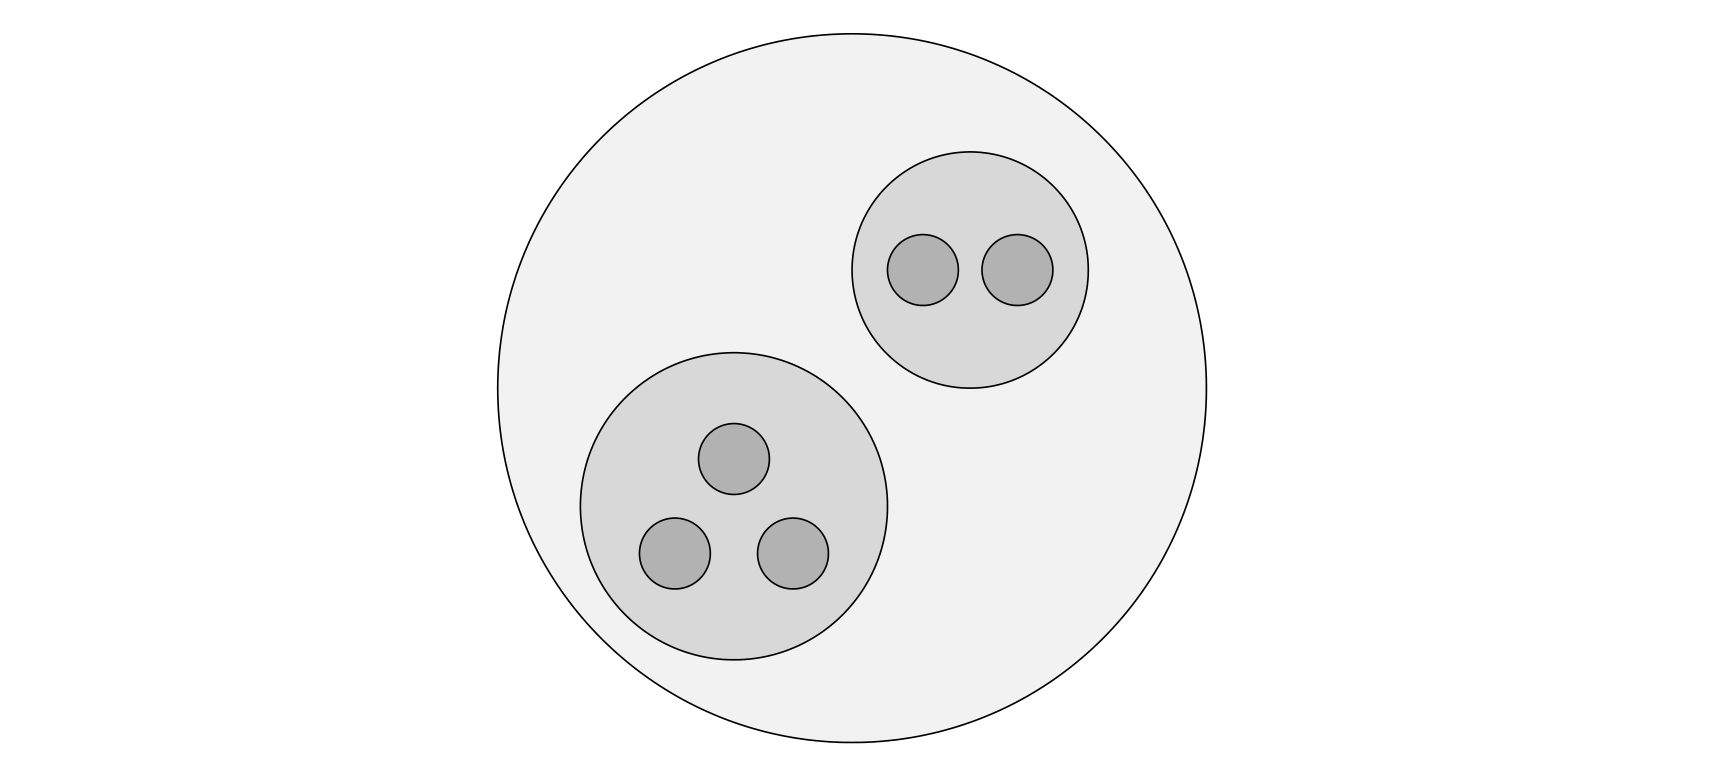
\includegraphics[width=0.42\textwidth]{figure11-1.png}
  \caption{一个二重乘法与一个三重乘法的复合给出一个五重乘法。（原文 p.~184，Figure 11.1）}
  \label{fig:11-1}
\end{figure}

\paragraph{题外话 5.}
应当把这与拓扑中如下论证作类比。对
\begin{equation}\tag{11.37}
f_1,f_2\in\pi_2(X)=\pi_0\bigl(\Omega^{2}X\bigr),
\end{equation}
我们可以想象红色部分被送到基点，并且
\begin{equation*}
\begin{array}{ccc}
\overset{f_1}{\bullet} & \simeq & \overset{f_2}{\bullet}\\[2pt]
 & \simeq & \\
\overset{f_2}{\bullet} & & \overset{f_1}{\bullet}
\end{array}
\end{equation*}
于是$\Gr$是$E_2$-空间。因此当我们把它线性化时，将得到一个$E_2$-对象。例如$\Shv(\Gr)$是$E_2$-范畴：它具有“弱交换”乘法。

\begin{srcrem}{72}
这对应着 3 维场论中线算子构成编织$\otimes$-范畴的方式。编织$\otimes$-范畴的范畴等价于$E_2$-范畴的范畴。
\end{srcrem}

也就是说，$\Gr$在 homotopy 理论的世界里有点像交换群。因此我们可以考虑某种拓扑层，例如局部系统，但我们需要更精细的东西，例如代数几何中会取的层。断言是：$\Gr$在代数几何的世界里也是某种交换群。这就是\term{因子化空间}{factorization space}的概念。

\begin{srcrem}{73}
眼下我们在曲线$C$上移动点，于是得到更大 2-圆盘中 2-圆盘的$E_2$-结构。但我们说过线算子其实更好：它们是$E_3$，因为我们多了一个时间维。然后当我们来到$\Gr$时，我们只看其模$G(\cO)$-作用的部分，即考虑
\begin{equation}\tag{11.38}
G(\cO)\backslash\Gr=G(\cO)\backslash\Gr/G(\cO),
\end{equation}
它实际上是$E_3$-空间，即比$E_2$更好。
\end{srcrem}

\begin{srcrem}{74}（警告）
我们忽略了$\Gr$的非约化结构。若$G$半单，则$\Gr$是约化的。即便是$\Gr_{GL_1}$，实际上也是$\Z\times$某个无穷维形式群。
\end{srcrem}

我们知道：
\begin{align}
\Gr_{GL_1}&=GL_1(K)/GL_1(\cO)\tag{11.39}\\
&=K^{*}/\cO^{*},\tag{11.40}
\end{align}
这里把二者都看成无穷维概形。由此我们应当有切空间
\begin{equation}\tag{11.41}
T\Gr_{GL_1}=\operatorname{Lie}(K^{*})/\operatorname{Lie}(\cO^{*})=K/\cO=\C((t))/\C[[t]],
\end{equation}
这是一个无穷维向量空间。一切交换，故$K/\cO$是无穷维 Lie 代数，于是可以指数化$\exp(K/\cO)$，得到无穷维形式群。于是
\begin{equation}\tag{11.42}
K^{*}/\cO^{*}\simeq\Z\times\exp(K/\cO),
\end{equation}
它大致是$\Z\times\bA^{\infty}$。

即便这对半单的$G$不出现，我们也不能忽略它。回忆$\operatorname{Pic}(C)=H^{1}(C,\cO^{*})$以及
\begin{equation}\tag{11.43}
T\operatorname{Pic}(C)=H^{1}(C,\cO)\simeq\cO(C\setminus x)\backslash K_x/\cO_x
\end{equation}
以及
\begin{equation}\tag{11.44}
K/\cO\twoheadrightarrow\cO(C\setminus x)\backslash K_x/\cO_x.
\end{equation}
于是我们有从$x$处的除子到 Pic 的映射：
\begin{equation}\tag{11.45}
K^{*}/\cO^{*}\to\operatorname{Pic},
\end{equation}
所以我们在$K_x/\cO_x$中忽略掉的多余部分，正是使 Pic 不离散的东西。

% [Tutor Note: (11.42) 中的$\bA^\infty$是形式无穷维仿射空间，原文 OCR 只留下 “$\Z\times$ d”，此处依 p.184 页面图恢复。(11.43) 的$T\operatorname{Pic}(C)=H^1(C,\cO)$是形式切空间，其右侧$\cO(C\setminus x)\backslash K_x/\cO_x$为“在$x$外正则的亚纯函数模去整函数”的商，切勿与$H^1$的 Zariski 切空间混淆。]

\subsection{$\Gr$的几何结构}\label{sec:11-2-2}

好的参考见 [PS86]。

我们首先要考虑的是$\Gr$的 Morse 理论/Bialynicki-Birula 分解/胞腔分解。分解的胞腔由到极大环面的同态标号，这些同态构成余权格：
\begin{equation}\tag{11.46}
\Bigl\{G_m\xrightarrow{\ \phi\ }T\subset G\Bigr\}=\Lambda.
\end{equation}
当我们有$G_m$的作用时便得到这样的分解。首先有来自旋转 Laurent 级数的$G_m\circlearrowright\Gr$。我们也可以在$T$内取一个一般的$G_m$拷贝：
\begin{equation}\tag{11.47}
G_m\xrightarrow{\ \rho^{\vee}\ }T\subset G.
\end{equation}
“一般”意味着中心化子$Z(\rho^{\vee})=T$。于是
\begin{equation}\tag{11.48}
G_m\to T\subset G\subset LG_+
\end{equation}
也作用在$\Gr$上。因此我们可以取对角作用，即同时旋转圆盘并作用这个$G_m$拷贝。

这个组合作用的不动点是什么？我们要找的是在两种作用下都不变的映射$D^{*}\to G\in G(K)$。因此不动点由余特征给出：
\begin{equation}\tag{11.49}
\{\phi\colon G_m\to T\}.
\end{equation}
这些可以限制到$D^{*}\subset G_m$，然后记住$T\subset G$。也就是说，我们有映射
\begin{equation}\tag{11.50}
\{\phi\colon G_m\to T\}\longrightarrow\{\phi\colon D^{*}\to G\},
\end{equation}
即余特征映到$\phi\in G(K)$，然后可以取相应的陪集。

\begin{srcex}{72}
对$GL_n$，我们考虑矩阵
\begin{equation}\tag{11.51}
\begin{pmatrix}
t^{i_1} & & & \\
 & t^{i_2} & & \\
 & & \ddots & \\
 & & & t^{i_n}
\end{pmatrix}\in GL_n(K).
\end{equation}
\end{srcex}
结论是：我们得到$\Gr$的一个胞腔分解，每个胞腔的中心恰有一个不动点。

我们其实已经见过这个余权格$\Lambda$。它是$T$的 Grassmann 流形：
\begin{equation}\tag{11.52}
\Lambda\simeq T(K)/T(\cO)=\Gr_T.
\end{equation}
也就是说：
\begin{equation}\tag{11.53}
\Lambda\cong\Gr_T\hookrightarrow\Gr_G.
\end{equation}
这是把非交换$G$的情形归约到交换$T$的情形的第一步。

下一步是找到 Cartan 分解。这些胞腔（不完全是同一回事，但）包含在$G(\cO)$-轨道之中。$\Gr$中的$G(\cO)$-轨道对应于$\Lambda$的点模 Weyl 群：
\begin{equation}\tag{11.54}
G(\cO)\backslash\Gr=LG_+\backslash LG/LG_+\leftrightarrow\Lambda/W\leftrightarrow\Lambda_+.
\end{equation}
背后还有一个仿射 Weyl 群$W_{\mathrm{Aff}}$，并且
\begin{equation}\tag{11.55}
\Lambda/W=W\backslash W_{\mathrm{Aff}}/W.
\end{equation}

% [Tutor Note: (11.54) 的最后一个双射$\Lambda/W\leftrightarrow\Lambda_+$需要先固定一个支配序（dominant chamber）；$\Lambda_+$指支配余权。$G(\cO)$-轨道与$LG_-$-轨道在$\Gr$上的偏序是相反的（见第 11.3 节与图 11.2），这是理解 (11.68) 中“集合相同但偏序反转”的关键。]

\section{$\Gr$中的轨道}\label{sec:11-3}

\begin{sectionkey}
本节把 Fourier 级数$\Vect^{\Z\text{-gr}}\simeq\Rep(G_m)$重释为$\Shv(\Gr_{GL_1})\simeq\QC(\Loc_{G_m}\PP^1)$，并指出对一般$G$应把左端换成$LG_+\backslash LG/LG_+$；后者作为集合与$\Bun_G(\PP^1)$相同，但闭包偏序相反，这一反差是后面分解定理的几何来源。
\end{sectionkey}

\begin{flushright}\small 第 27 讲；2021 年 5 月 4 日\end{flushright}

几何 Satake 对应是 Fourier 级数理论的非交换对应物。回忆 Fourier 级数理论给出识别
\begin{equation}\tag{11.56}
\Vect^{\Z\text{-gr}}\simeq\Rep(G_m).
\end{equation}
然后我们把左端识别为
\begin{equation}\tag{11.57}
\Vect^{\Z\text{-gr}}\simeq\Shv(\Gr_{GL_1}),
\end{equation}
并把右端识别为
\begin{equation}\tag{11.58}
\Rep(G_m)\simeq\QC(\mathrm{pt}/G_m)\simeq\QC\bigl(\Loc_{G_m}\PP^1\bigr).
\end{equation}
目前我们忽略导出结构，因为一切皆交换。于是 Fourier 级数的重新解释是
\begin{equation}\tag{11.59}
\Shv(\Gr_{GL_1})\simeq\QC\bigl(\Loc_{G_m}\PP^1\bigr),
\end{equation}
而我们要把左端换成关于$G$的仿射 Grassmann 流形的表述：
\begin{equation}\tag{11.60}
\Gr_G=G(K)/G(\cO)=LG/LG_+.
\end{equation}
但我们只关心（其上的层）模$G(\cO)$-作用的情形，即关心轨道：
\begin{align}
G(\cO)\backslash\Gr_G&{}\tag{11.61}\\
&=G(\cO)\backslash G(K)/G(\cO)\tag{11.62}\\
&=LG_+\backslash LG/LG_+.\tag{11.63}
\end{align}
回忆我们在物理中把它看成意大利饺（ravioli）上的$G$-丛空间：
\begin{equation}\tag{11.64}
LG_+\backslash\Gr_G=LG_+\backslash LG/LG_+=\Bun_G\bigl(\text{意大利饺}\bigr).
\end{equation}
我们有
\begin{equation}\tag{11.65}
\Bun_G\bigl(\text{意大利饺}\bigr)=\Bun_G(\PP^1),
\end{equation}
并且可以把$\PP^1$看成一个 2-球面，由圆盘$D$与一份去掉原点的$\bA^1$粘成。于是$LG_+$可以看成圆盘上丛的自同构，但我们还需要模掉$\bA^1$上平凡化的改变，即模掉映射$\bA^1\to G$：
\begin{equation}\tag{11.66}
LG_-=\{\bA^1\to G\}.
\end{equation}
因此
\begin{equation}\tag{11.67}
LG_-\backslash LG/LG_+=\Bun_G(\PP^1).
\end{equation}
于是意大利饺与$\PP^1$在拓扑上看起来非常相似，且意大利饺上丛的同构类与$\PP^1$上丛的同构类一一对应。也就是说，我们有双射
\begin{equation}\tag{11.68}
LG_+\backslash LG/LG_+\leftrightarrow\Lambda/W\leftrightarrow\Bun_G\PP^1,
\end{equation}
其中$\Lambda=\Hom(G_m,T)$是余权格。所以二者作为集合相同，但偏序结构非常不同。$LG_+\circlearrowright\Gr$的轨道在闭包关系下构成一个偏序集。这些轨道都是有限维的，且每个轨道的闭包中只有有限多个轨道。另一方面，$\Bun_G\PP^1$作为集合与之相同，但偏序是反过来的。

\begin{srcex}{73}
让我们考虑$G=GL_2$。第一 Chern 类是映射
\begin{equation}\tag{11.69}
\Bun_{GL_2}(\PP^1)\to\Z.
\end{equation}
例如$\deg(\cO\oplus\cO)=0$，而$\deg(\cO\oplus\cO(1))=1$。$\Bun_{GL_2}(\PP^1)$不连通，其连通分支由度数相同的丛组成，即对每个$n\in\Z$有一个分支。
\end{srcex}

考虑度数为$0$的丛。它等同于$SL_2$-丛：
\begin{equation}\tag{11.70}
\Bun_{SL_2}(\PP^1)=\deg^{-1}(0).
\end{equation}

\begin{figure}[htbp]
  \centering
  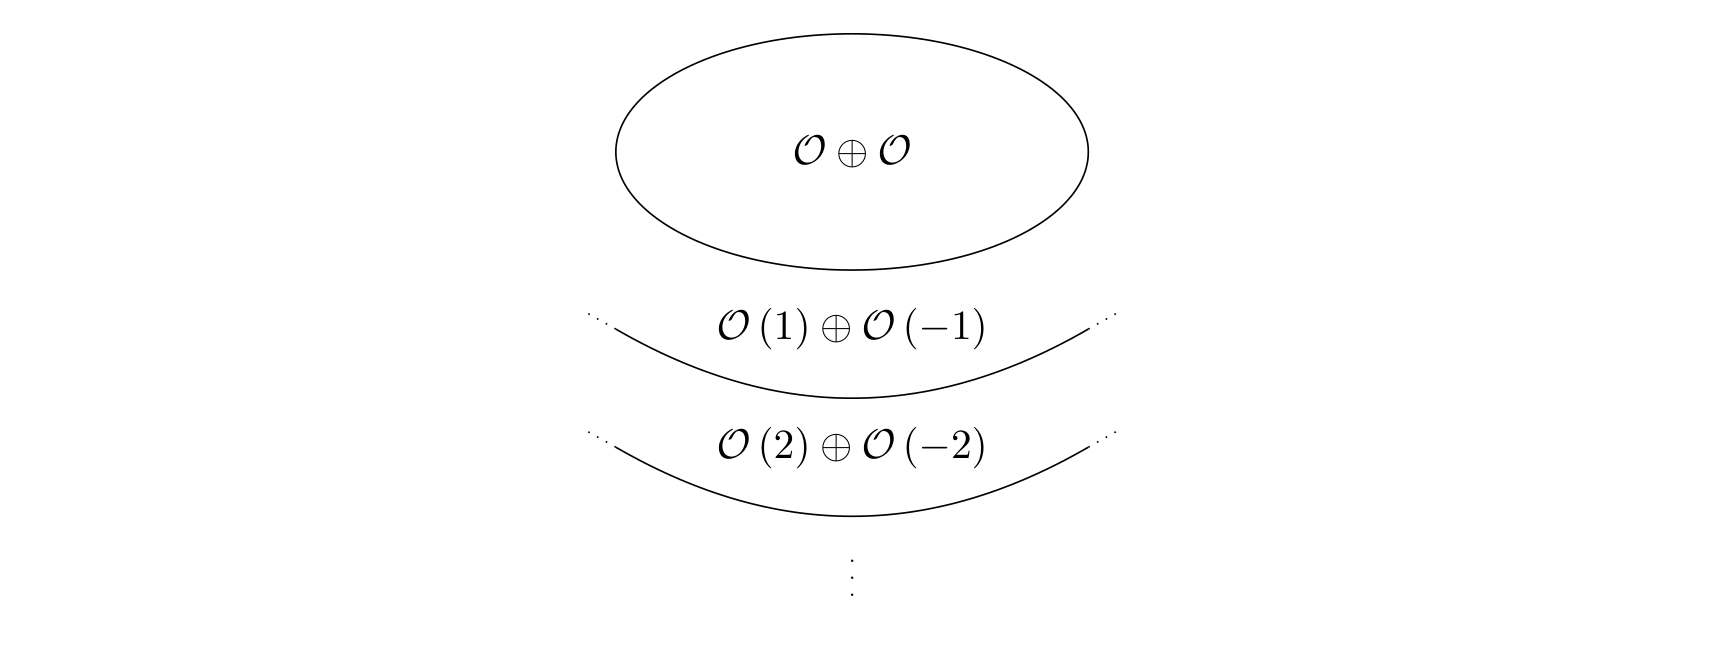
\includegraphics[width=0.5\textwidth]{figure11-2.png}
  \caption{包含平凡丛的$\Bun_{GL_2}(\PP^1)$连通分支有一个开稠密轨道。图中各层对应其他 stratum，它们必然包含在中心开 stratum 的闭包中。我们也可以把此图看作$\Gr$上$LG_-$-轨道的图像。（原文 p.~188，Figure 11.2）}
  \label{fig:11-2}
\end{figure}

这里有平凡丛$\cO\oplus\cO$，以及其他丛如$\cO(1)\oplus\cO(-1)$。这是一个连通空间，含有一个包含$\cO\oplus\cO$的开稠密 stratum。所以所有其他 stratum 都包含在平凡丛所在 stratum 的闭包中。于是偏序看起来像$\mathbb{N}$。

如图 11.2 所示。$\Gr$上的偏序结构是相反的：有一个闭轨道包含在其他一切的闭包之中。

我们也可以把图 11.2 看作$\Gr$中$LG_-$-轨道的图像：有一个开轨道，且所有轨道都是有限余维的。这与$\Gr$中$LG_+$-轨道的情形相反——那里轨道是有限维的，且闭包关系方向相反。

% [Tutor Note: (11.68) 中第二个双射严格地说应写成$LG_+\backslash LG/LG_+\leftrightarrow\Bun_G(\PP^1)$的同构类集合，而非$\Bun_G\PP^1$本身；原文以同一记号兼指模空间与其点集，译文从之。此处的$\Lambda/W$与$LG_-$-轨道的对应关系依赖$LG_-\backslash LG/LG_+$的分解，与$LG_+$-轨道的$\Lambda_+$标号相差一个支配序取反。]

\section{$\Gr$上的等变层}\label{sec:11-4}

\begin{sectionkey}
本节引入核心范畴$\sph=\Shv_{LG_+}(\Gr_G)$：它是半单的，简单对象由$\Lambda/W$标号；其上同时有来自双陪集的结合乘法和来自因子化的编织乘法，二者经 Eckmann–Hilton 论证合成对称幺半结构。
\end{sectionkey}

在$\Gr_G$内部我们有余权格
\begin{equation}\tag{11.71}
\Lambda\simeq\Gr_T\subset\Gr_G,
\end{equation}
它作为“胞腔中心”坐落，即作为$G_m$-作用的不动点。再次，$LG_+\backslash\Gr_G$与$\Lambda/W$一一对应。而$\Lambda/W$看起来像是某个群$G^{\vee}$的不可约表示，该群的极大环面$T^{\vee}$对偶于$T$，也就是说
\begin{equation}\tag{11.72}
\Lambda=\Hom(T^{\vee},G_m).
\end{equation}
我们将从$\Gr_G$上的$LG_+$-等变层出发（用 Tannakian 方法）重构这个对偶群$G^{\vee}$：
\begin{equation}\tag{11.73}
\sph=\Shv_{LG_+}(\Gr_G).
\end{equation}
这里的$\Shv$指 D-模的阿贝尔范畴，或所谓的反常层（perverse sheaf）范畴。想法是：在每个轨道上，这些层将是带平坦联络的向量丛，或等价地，是平移了轨道维数后的局部系统。

这两类范畴都有简单对象，它们与轨道上的不可约局部系统一一对应。$LG_+$-轨道并不完全是胞腔，但被胞腔铺砌（paved）。特别地，所有$LG_+$-轨道都是单连通的。事实上我们可以把它们显式地描述为$G$的部分旗流形上的仿射丛。这意味着$\sph$中的简单对象与轨道$\Lambda/W$一一对应。

结果是：$\sph$是半单范畴，即每个对象都是单对象的直和。这与维数的奇偶性有关，即各轨道复维数的奇偶性在每个连通分支上为常数。要点在于，这限制了一个轨道上的层与其闭包中轨道上的层之间可能的交互：闭包中的轨道与之相差复余维$2$。这意味着不存在可能的扩张，即对不同轨道上的层有$\operatorname{Ext}^{1}=0$。

结论是：这个范畴非常简单，每个对象都是按轨道标号的对象之直和，即作为抽象范畴有
\begin{equation}\tag{11.74}
\sph\simeq\Vect(\Lambda/W).
\end{equation}
\footnote{识别$\sph\simeq\Vect(\Lambda/W)$并不是一个自然的识别。特别地，$\sph$是幺半的，而$\Vect(\Lambda/W)$在幺半结构意义下是一个糟糕的模型。}
这很好，因为这正是一个约化群的表示范畴的样子。

回忆紧群在 Pontryagin 对偶下对偶于离散群。当我们讨论 Tannakian 版本时，我们看到约化群对偶于半单范畴。所以这种对偶暗示：当我们有某种离散性/半单性时，对偶一侧将涉及某个复约化群之类的东西。

主要的结构是：$\sph$是对称幺半范畴，即它有交换张量积。我们从线算子的角度解释了这一点。这有两种不同的结构，它们以某种精确的方式相容。第一种是来自双陪集上层的结构：
\begin{equation}\tag{11.75}
\Shv(LG_+\backslash LG/LG_+).
\end{equation}
双陪集空间上的层总有一个结合乘法。

还有另一种结构，它类似于编织乘法，来源完全不同。特别地，我们看到$\Gr_G$在取商之前就有乘法结构。也就是说，在同伦意义下
\begin{equation}\tag{11.76}
\Gr_G=\Omega^{2}(BG),
\end{equation}
这赋予它弱交换乘法。在代数几何中我们必须换一种说法，用到 Beilinson–Drinfeld 的因子化概念。

\subsection{因子化结构}\label{sec:11-4-1}

$\Gr_G$有某种阿黛尔版本，它是$\Omega^{2}(BG)$上$E_2$-结构的代数几何版本。随后 Beilinson–Drinfeld 引入了 BD Grassmann 流形。想法是：Grassmann 流形相互拼合的方式编码了某种乘法结构。

固定一条曲线$C$（例如$C=\bA^1,\PP^1$，或任取\footnote{曲线不影响最终答案。}）。然后我们将对所有的$n$定义生活在$C^{n}$上的对象$\Gr_{G,C^{n}}$：
\begin{equation}\tag{11.77}
\begin{array}{ccc}
\Gr_{G,C^{n}} & & \\
\downarrow & & \\
C^{n} & &
\end{array}
\end{equation}
如下所述。对$n=1$这是
\begin{equation}\tag{11.78}
\begin{array}{ccc}
\Gr_{G,C} & & \\
\downarrow & & \\
C & &
\end{array}
\end{equation}
其中$x\in C$上的纤维由$C$上的$G$-丛连同$C\setminus x$上的平凡化构成。于是我们有$\Gr$的这个解释：在原点之外有平凡化的丛。接着 Beilinson–Drinfeld 让原点取任意点$x$，最终得到$C$上的这个丛。$\Gr_{G,C}$是$\Gr_G$上由圆盘上平凡化的改变作用所给出的伴随丛：$\Aut(D)\circlearrowright\Gr_G$。

对$n=2$，
\begin{equation}\tag{11.79}
\begin{array}{ccc}
\Gr_{G,C^{2}} & & \\
\downarrow & & \\
C^{2} & &
\end{array}
\end{equation}
$(x,y)\in C^{2}$上的纤维由$C$上的$G$-丛连同$C\setminus\{x,y\}$上的平凡化构成。注意，尽管$(x,y)$是有序对，该构造在对称群作用下不变。真正有趣的是$C^{2}$中有两个 stratum。我们有开 stratum
\begin{equation}\tag{11.80}
C^{2}\setminus\Delta=\{x\ne y\},
\end{equation}
在它上面
\begin{equation}\tag{11.81}
\Gr_{G,C^{2}}\big|_{x,y}\simeq\Gr_{G,C}\big|_{x}\times\Gr_{G,C}\big|_{y},
\end{equation}
于是有
\begin{equation}\tag{11.82}
\Gr_{G,C^{2}}\big|_{C^{2}\setminus\Delta}\simeq\Gr_{G,C}\big|^{\times 2}_{C^{2}\setminus\Delta}.
\end{equation}
若我们看另一个 stratum
\begin{equation}\tag{11.83}
\{x=y\}=\Delta\subset C^{2},
\end{equation}
则
\begin{equation}\tag{11.84}
\Gr_{G,C^{2}}\big|_{x,y}\simeq\Gr_{G,C}\big|_{x},
\end{equation}
于是
\begin{equation}\tag{11.85}
\Gr_{G,C^{2}}\big|_{\Delta}\simeq\Gr_{G,C}.
\end{equation}

\begin{srcex}{74}
对$G=GL_1$，我们在对角线之外有$\Z\times\Z$，在对角线上有$\Z$。也就是说，我们有$\Z\times\Z\times C^{2}\setminus\Delta$与对角线上的$\Z\times C$粘在一起。粘合映射就是整数的群律。
\end{srcex}

我们可以把这看成群的动态写法。给定两个群元素$(n,m)\in\Z\times\Z$，我们可能想知道它们如何相加。于是我们考虑把$n$放在点$x$，把$m$放在点$y$，并让这两点碰撞。那么$\Gr_{GL_1,C^{n}}$的几何就编码了加法律。也就是说，群结构由$\Z\times\Z$（对角线之外）与$\Z$（对角线上）之间的粘合映射显式呈现。

所以一般而言我们有这个族$\Gr_{G,C^{n}}$，它具有以下两个关键结构。

\begin{enumerate}
\item $\Gr_{G,C^{n}}\big|_{\{x_i\}_{i=1}^{n}}$只依赖于子集$\{x_i\}\subset C$。即对有限集的满射$I\twoheadrightarrow J$我们得到相应的对角映射$\Delta_{I\twoheadrightarrow J}$，并且
\begin{equation}\tag{11.86}
\Delta^{*}_{I\twoheadrightarrow J}\Gr_{C}^{I}\simeq\Gr_{C}^{J}.
\end{equation}
例如$\Delta^{*}\Gr_{C}^{2}\simeq\Gr_{C}$。我们可以换一种说法：$\Gr_{C}(-)$定义了某个有限子集空间上的族，该空间称为$C$的 Ran 空间：
\begin{equation}\tag{11.87}
\operatorname{Ran}(C)=\operatorname{colim}_{I\twoheadrightarrow J}C^{I},
\end{equation}
即$C$的有限子集的参数空间。

\item 因子化：$\Gr$关于不交并运算是乘性的。即
\begin{equation}\tag{11.88}
\Gr_{G,C^{m+n}}\big|_{\{x_i\}_{i=1}^{m}\sqcup\{y_i\}_{i=1}^{n}}\simeq\Gr_{G,C^{m}}\big|_{\{x_i\}_{i=1}^{m}}\times\Gr_{G,C^{n}}\big|_{\{y_i\}_{i=1}^{n}}.
\end{equation}
\end{enumerate}

\begin{srcrem}{75}
在拓扑中我们有一个真正的乘法映射：对从带点圆盘到$BG$的两个映射，我们可以把它们看作生活在更大的圆盘中。现在我们有例如$C$中的两个点，并且可以取它们碰撞的极限。结果来自两份 Grassmann 流形（在$\Delta$之外）与一份 Grassmann 流形（沿$\Delta$）之间的粘合。
\end{srcrem}

这就是所谓的因子化空间。它编码了$\Gr$上不寻常的代数结构，该结构在 homotopy 范畴中退化为$E_2$-结构。它定义了$\Gr$上对象（例如层等）的乘法，我们可以取极限。例如，给定$\cF,\cG\in\Shv(\Gr_G)$以及$x,y\in C=\bA^1$，我们可以认为$\cF$生活在$x$处、$\cG$生活在$y$处：
\begin{equation}\tag{11.89}
\cF\in\Shv\bigl(\Gr_{G,C}|_{x}\bigr),\qquad \cG\in\Shv\bigl(\Gr_{G,C}|_{y}\bigr),
\end{equation}
这定义了一个层
\begin{equation}\tag{11.90}
\cF\boxtimes\cG\in\Shv\Bigl(\Gr_{G,C^{2}}\big|_{C^{2}\setminus\Delta}\Bigr).
\end{equation}
现在我们要取$x\to y$的极限，即要把这个构造延拓到对角线上。若这些层是例如凝聚层，我们就做不到这一点。但若这些层足够接近拓扑层，那就走运了：构造邻近循环（nearby cycles）正是这种极限的拓扑版本。于是我们可以把$\cF*\cG$定义为$\cF\boxtimes\cG$在$\Delta\subset C^{2}$上的邻近循环。

因此$\Shv(\Gr)$大致看起来像$E_2$/编织$\otimes$-范畴，但邻近循环的构造并不恰好给出结合的张量积。然而，若我们限制到$\Gr$上的$LG_+$-等变层，就得到
\begin{equation}\tag{11.91}
\sph=\Shv_{LG_+}(\Gr)
\end{equation}
上的结合、编织张量结构。

我们可以这样理解。我们可以“竖直地”堆叠修正（这是 Hecke 结构），也可以在不同点处作修正并把它们碰撞。于是有三个乘法方向：结合的竖直方向，以及来自碰撞的编织乘法。由 Eckmann–Hilton 论证，这定义了一个交换乘法，即范畴上的对称幺半结构。我们在物理中已经见过这一点：我们研究的是余维$1$缺陷，即$C\times I$中的点，而来自碰撞点/把小球碰进大 3-球所得的乘法是交换的，因为我们有足够的维数让它们互相绕行。

% [Tutor Note: (11.74) 的半单性依赖于系数域特征为$0$（D-模范畴）或$\Q_\ell$-层、且轨道维数奇偶性恒定；若在正特征或整系数下，$\operatorname{Ext}^1$未必消失。(11.88) 的因子化同构必须在$\{x_i\}\cap\{y_i\}=\varnothing$时陈述；在对角线附近应改为邻近循环/因子化范畴的陈述，这正是原文随后讨论的内容。]

\section{$\sph$的 Tannakian 重构}\label{sec:11-5}

\begin{sectionkey}
本节说明如何用 Tannakian 形式重构$G^{\vee}$：先构造$\sph\to\Shv(\Gr_T)\simeq\Rep(T^{\vee})$，再对$\Vect$取纤维函子；并指出$\Spec(\sph)$自然接收$\mathrm{pt}/T^{\vee}\to\Spec(\sph)$。
\end{sectionkey}

回忆 Tannakian 重构从一个对称幺半范畴$(\cC,*)$出发。然后我们给它配上叠$\Spec(\cC,*)$。对足够好的$\cC$，想法是
\begin{equation}\tag{11.92}
\cC\simeq\QC(\Spec(\cC,*)).
\end{equation}
还有一个（可能更熟悉的）变体，其中我们多带一点数据。若我们有$(\cC,*)$连同一个纤维函子（忠实且正合的$\otimes$-函子）
\begin{equation}\tag{11.93}
(\cC,*)\to(\Vect_k,\otimes),
\end{equation}
则这给出一个映射
\begin{equation}\tag{11.94}
\Spec(\Vect_k,\otimes)=\Spec(k)\longrightarrow\Spec(\cC,*),
\end{equation}
它是平坦覆盖。这意味着
\begin{equation}\tag{11.95}
\Spec(\cC,*)\xrightarrow{\ \simeq\ }\mathrm{pt}/\Gal(\cC,F),
\end{equation}
其中
\begin{equation}\tag{11.96}
\Gal(\cC,F)=\Aut(F).
\end{equation}
所以在我们这里需要某个遗忘函子
\begin{equation}\tag{11.97}
\sph=\Shv_{LG_+}(\Gr)\to\Vect.
\end{equation}
说明这一点最简短但也许最缺乏洞见的说法是：这就是上同调函子。我们将采取不同的途径。首先考虑函子
\begin{equation}\tag{11.98}
\sph=\Shv_{LG_+}(\Gr_G)\to\Shv(\Gr_T).
\end{equation}
这很有用，因为
\begin{equation}\tag{11.99}
\Gr_T\simeq\Lambda,
\end{equation}
于是我们直接做 Fourier 级数：
\begin{equation}\tag{11.100}
\Shv(\Gr_T)\simeq\Shv(\Lambda)\simeq\Rep(T^{\vee}),
\end{equation}
其中$T^{\vee}=\Hom(\Lambda,G_m)$。所以通过把$\Gr_G$与$\Gr_T$联系起来，我们将得到一个不只到$\Vect_k$的函子，而是
\begin{equation}\tag{11.101}
\sph\to\Rep(T^{\vee}).
\end{equation}
我们如何把$\Gr_G$与$\Gr_T\simeq\Lambda$联系起来？在 Grassmann 流形内部有$G_m$-作用的不动点：
\begin{equation}\tag{11.102}
\Lambda\hookrightarrow\Gr_G.
\end{equation}
于是我们想把$\Gr_G$上的层对应为对$\Lambda$的每个点附一个向量空间，即对每个胞腔中心的不动点附一个向量空间。

我们接下来会讨论抛物限制，但要点是：我们可以通过穿过$\Gr_B$把$\Gr_G$上的层与$\Gr_T\simeq\Lambda$上的层联系起来：
\begin{equation}\tag{11.103}
\begin{array}{ccc}
 & \Gr_B & \\
 \swarrow & & \searrow\\
 \Gr_G & & \Gr_T
\end{array}
\end{equation}
其中$B$是 Borel：
\begin{equation}\tag{11.104}
G\supset B\twoheadrightarrow T.
\end{equation}
\begin{srcex}{75}
若$G=GL_n$，则$B$由上三角矩阵组成。于是对角矩阵组成$T$，它由$B$模严格上三角矩阵的商给出。
\end{srcex}
于是我们得到一个漂亮的忠实$\otimes$-函子$\sph\to\Rep(T^{\vee})$，它可以限制到$\Vect_k$得到忠实的$\otimes$-函子：
\begin{equation}\tag{11.105}
\begin{array}{ccc}
 & \sph & \\
 \swarrow & & \searrow\\
\Rep(T^{\vee}) & \xrightarrow{\ \operatorname{Forget}\ } & \Vect_k
\end{array}
\end{equation}
但最终，这幅图景将告诉我们：事实上$\Spec(\sph)$自然地接收一个映射
\begin{equation}\tag{11.106}
\mathrm{pt}/T^{\vee}\longrightarrow\Spec(\sph).
\end{equation}

% [Tutor Note: (11.95) 中的箭头方向是$\Spec(\cC,*)\simeq\mathrm{pt}/\Gal(\cC,F)$，即把 Tannakian 叠实现为“纤维函子的自同构群”的分类空间；原文排版把$\simeq$与箭头叠在一起，译文按语义写成$\xrightarrow{\simeq}$。(11.100) 的$\Shv(\Lambda)\simeq\Rep(T^{\vee})$是 Fourier 变换（每点取纤维再对格作 Fourier），需要$\Lambda$为有限生成自由交换群。]

\section{抛物诱导/抛物限制}\label{sec:11-6}

\begin{sectionkey}
本节把最高权理论几何化：用对应$\mathrm{pt}/B\rightleftarrows\mathrm{pt}/G,\mathrm{pt}/T$定义抛物限制（取$N$-不变量）与抛物诱导（$G/B$上截面），并把它搬到$\Gr_B\to\Gr_G,\Gr_T\simeq\Lambda$上，得到 Mirkovi\'c–Vilonen 半无限轨道与几何 Satake 的纤维函子。
\end{sectionkey}

\begin{flushright}\small 第 28 讲；2021 年 5 月 6 日\end{flushright}

\subsection{对约化群}\label{sec:11-6-1}

我们想要一种有意义的方式，把复约化群$G$的表示与极大环面$T$的表示联系起来。这是最高权理论的一个版本。回忆我们可以用最高权理论研究$G$的有限维表示。回顾如下。固定一个 Borel $B\subset G$，即子群$B\subset G$使得$G/B$是$G$的极大射影商。\footnote{等价地，Borel 可定义为$G$的极大 Zariski 闭、连通的可解代数子群。}这个商$\cB=G/B$是$G$的旗簇。在$B$内部我们可以考虑换位子群
\begin{equation}\tag{11.107}
N:=[B,B]\subset B,
\end{equation}
然后取商，得到一个环面：
\begin{equation}\tag{11.108}
T=B/N.
\end{equation}

\begin{srcex}{76}
若$G=GL_n$，则$B$由上三角矩阵组成，$N$由严格上三角矩阵组成，而$T=B/N$由对角矩阵组成。
\end{srcex}

\begin{srcrem}{76}
人们最初可能把环面$T$当作$G$的子群来认识，但更有用的想法是把它看成一个商：
\begin{equation}\tag{11.109}
G\supset B\twoheadrightarrow T.
\end{equation}
\end{srcrem}

现在我们可以构造$\mathrm{pt}/B$，它定义一个对应：
\begin{equation}\tag{11.110}
\begin{array}{ccc}
 & \mathrm{pt}/B & \\
 \swarrow & & \searrow\\
 \mathrm{pt}/G & & \mathrm{pt}/T
\end{array}
\end{equation}
它通过推-拉（push-pull）定义了$\mathrm{pt}/G$与$\mathrm{pt}/T$的线性化（即$G$与$T$的表示）之间的态射。具体地，对$V\in\Rep(G)$，我们可以把它拉回到$\mathrm{pt}/B$得到
\begin{equation}\tag{11.111}
V|_{B}\in\Rep(B).
\end{equation}
然后我们可以把它前推到$\mathrm{pt}/T$。为了看清这是什么，让我们把图景稍微丰富一下，取映射$\mathrm{pt}/B\to\mathrm{pt}/T\leftarrow\mathrm{pt}$的纤维积，得到
\begin{equation}\tag{11.112}
\begin{array}{ccc}
\mathrm{pt}/N & \longrightarrow & \mathrm{pt}/B\\
\downarrow & & \downarrow\\
\mathrm{pt} & \longrightarrow & \mathrm{pt}/T
\end{array}
\end{equation}
因此，从$\mathrm{pt}/B$前推到$\mathrm{pt}/T$，在底层向量空间层面就是从$\mathrm{pt}/N$前推到$\mathrm{pt}$，即取$N$-不变量。于是从$V\in\Rep(G)$出发得到
\begin{equation}\tag{11.113}
\bigl(V|_{B}\bigr)^{N}\in\Rep(T).
\end{equation}
对表示$V$取$N$-不变量给出经典意义上的$V$的最高权向量。$T$的作用就是最高权。

这称为\term{抛物限制}{parabolic restriction}。

注意，这不是从$G$到$T\subset G$的朴素限制，而是把$T$看成$B$的商，并用$\mathrm{pt}/B$作为对应把它们联系起来。它有一个伴随，称为\term{抛物诱导}{parabolic induction}，把一个$T$-表示变成一个$G$-表示，如下所述。

注意映射$\mathrm{pt}/B\to\mathrm{pt}/G$的纤维是旗簇$G/B$。设$C_\lambda$是$T$按某特征$\lambda$作用的一维向量空间。当把它拉回到$\mathrm{pt}/B$时，我们得到
\begin{equation}\tag{11.114}
\mathrm{pt}/B=G\backslash G/B
\end{equation}
上的层，于是$\mathrm{pt}/G$上的层等价于$G/B$上的$G$-等变向量丛$L_\lambda$。然后前推得到
\begin{equation}\tag{11.115}
\Gamma(G/B,L_\lambda)\in\Rep(G).
\end{equation}
这就是最高权表示的经典构造。

\begin{srcrem}{77}
我们可以更抽象地思考这幅图。以$G$为规范群的规范理论是关于映入$\mathrm{pt}/G$的映射的理论，即关于任意空间上$G$-丛的理论。研究$G$-丛时，自然要找约化到$B$（即旗）的约化，然后看相应的$T$-丛。于是这把$G$-丛的理论与$T$-丛的理论联系了起来。我们最终会把它解释为$G$-规范理论与$T$-规范理论之间的一个界面。
\end{srcrem}

现在我们可能想知道，若先做抛物诱导再做抛物限制会怎样，即这一程序给出$\mathrm{pt}/T$的线性化的哪些对称性。复合这些对应，我们看到作为对称性作用的自然对象是纤维积$B\backslash G/B$：
\begin{equation}\tag{11.116}
\begin{array}{ccc}
B\backslash G/B & \longrightarrow & \mathrm{pt}/B\\
\downarrow & & \downarrow\\
\mathrm{pt}/B & \longrightarrow & \mathrm{pt}/G
\end{array}
\end{equation}
即它是 Bruhat 胞腔，集合论上与 Weyl 群一一对应。因此这幅抛物诱导图景的对称性由有限 Hecke 代数给出。

\subsection{对$\Gr_G$}\label{sec:11-6-2}

做这一切的目的是把$G$-规范理论与我们已理解的东西联系起来。思路是：为了研究$\Gr_G$上的层，我们应试着把它们与$\Gr_T$上的层联系起来。

我们已经看到$\Gr_T$是一个格，$\Gr_T\simeq\Lambda$，而且事实上$\Gr_T\simeq\Lambda\hookrightarrow\Gr_G$。但我们不应只作朴素限制。

\begin{srcrem}{78}
除非另有说明，当你试图把$G$与$T$作比较时，应始终使用抛物限制，而不是朴素限制。
\end{srcrem}

基本想法是，我们将有
\begin{equation}\tag{11.117}
\begin{array}{ccc}
 & \Gr_B & \\
 p\swarrow & & \searrow q\\
 \Gr_G & & \Gr_T\simeq\Lambda
\end{array}
\end{equation}
而我们要的基本函子将形如
\begin{equation}\tag{11.118}
q_{*}p^{!}\colon\sph_G\to\sph_T\simeq\Rep(T^{\vee}).
\end{equation}

\subsection{$\Gr_B$}\label{sec:11-6-3}

我们已经看到$\Gr_T$只是一个格，随后又讨论了$\Gr_G$的结构。现在我们来理解$\Gr_B$。这将与约化群情形非常不同，因为$B$可解。按定义
\begin{equation}\tag{11.119}
\Gr_B=B(K)/B(\cO).
\end{equation}
例如我们看的是 Laurent 级数中的上三角矩阵模去 Taylor 级数中的上三角矩阵。我们真正感兴趣的是双陪集栈
\begin{equation}\tag{11.120}
\Gr_B:=B(\cO)\backslash\Gr_B=B(\cO)\backslash B(K)/B(\cO).
\end{equation}
回忆$\Gr_G$由$C\setminus\mathrm{pt}$上有平凡化的$G$-丛组成。$\Gr_B$类似地由$C\setminus\mathrm{pt}$上有平凡化的$B$-丛组成。关键的观察是：$G$-丛的平凡化比把结构群约化到$B$要强得多。要点在于，约化到$B$是给一个完整旗，而若你有平凡化，你就可以直接把坐标子空间取作旗。因此，给定在一点之外有平凡化的$G$-丛，它当然在点之外有到$B$的约化。也就是说，我们得到一个从$C\setminus\mathrm{pt}$到参数化$\C^{n}$中旗的空间的映射，即一个映射$C\setminus\mathrm{pt}\to G/B$。

于是对$P\in\Gr_G$，我们得到$C\setminus\mathrm{pt}$上伴随$G/B$-丛$P\times^{G}G/B$的一个截面。现在我们有一个美妙的东西，称为真性的赋值判别法（valuative criterion of properness），它说：若我有一个从去心曲线出发的映射$D^{*}\to G/B$，则它唯一地延拓为整个圆盘上的映射$D\to G/B$。注意这不是族中的陈述，而是域上的陈述。

所以断言如下。

\begin{srcclaim}{2}
在$k$-点层面，$\Gr_B\to\Gr_G$是双射。
\end{srcclaim}

这不是族中的陈述，即这并非说这些空间不同胚。事实上我们可以如下实现它。无论$\Gr_B$是什么，它都映到$\Gr_G$和$\Gr_T$，而后者完全不连通（$\Gr_T\simeq\Lambda$）。因此
\begin{equation}\tag{11.121}
\Gr_B=\bigsqcup_{\lambda\in\Lambda}\Gr_{B,\lambda},
\end{equation}
即我们把$\Gr_B$撕成了以$\lambda\in\Lambda$标号的块。

图景如下。回忆$\Gr_G$上有$G(\cO)$-轨道，其中包含对应于$\Lambda$中点的$G(\cO)$-不动点。于是，集合论上$\Gr_G$是以$\lambda\in\Lambda$标号的块$S_\lambda$的不交并，$S_\lambda$是$\lambda\in\Lambda$在$\Gr_G$中的原像。再次，由于$T=B/N$，我们有
\begin{equation}\tag{11.122}
\begin{array}{ccc}
\mathrm{pt}/N & \longrightarrow & \mathrm{pt}/B\\
\downarrow & & \downarrow\\
\mathrm{pt} & \longrightarrow & \mathrm{pt}/T
\end{array}
\end{equation}

\paragraph{习题 3.}
用此证明$S_\lambda$恰好是$LN=N(K)$的轨道。

这些轨道称为\term{半无限轨道}{semi-infinite orbits}。这些轨道是无穷维的，但同时也是无穷余维的。

% [Tutor Note: Claim 2 只在$k$-点（甚至只在代数闭域的点）上成立；$\Gr_B\to\Gr_G$在族中既非单射也非满射，因此不能据此断言二者作为 ind-概形同构。习题 3 中$N(K)$的轨道$S_\lambda$与$G(\cO)$-轨道方向相反：前者无穷维、有限维截面的余维无穷，这正是 MV 循环的支撑。]

\subsection{几何 Satake 定理}\label{sec:11-6-4}

以上全部内容的结论是，我们有一个函子
\begin{equation}\tag{11.123}
\sph_T\simeq\Rep(T^{\vee})\xleftarrow{\ \text{对 }N(K)\text{-轨道的 }!\text{-限制的上同调}\ }\sph_G.
\end{equation}
也就是说，我们从$G\in\sph_G$出发，结果是一个$\Lambda$-分次向量空间。我们可以就此打住，也可以与$\operatorname{Forget}\colon\Rep(T^{\vee})\to\Vect$复合，得到一个真正的纤维函子。这就是几何 Satake 对应的正确纤维函子。

它显然是张量函子，因为我们用来构造它的运算都与因子化结构（碰撞点）以及由双陪集实现的对称性相容。它也（相当）显然是忠实的。想法是：我们考虑层$\cF\in\Shv(G(\cO)\backslash\Gr)$，该层支撑在某个 stratum 的闭包上。在这个极大轨道内部选一个不动点$\lambda$；若我们通过限制到$S_\lambda$来做这个测量，则基本得到该点处的 stalk。

在较低的 stratum 上测量会更复杂，但我们至少可以挑出$\cF$支撑的顶维部分，并用它来检验函子是忠实的。

于是我们得到几何 Satake 定理。$\Gr$拓扑中的基本几何现象由 Lusztig 识别，Ginzburg 把它表述成今天的形式（并勾画了证明），随后 Drinfeld 引入了因子化图景，最后 Mirkovi\'c–Vilonen 引入了这些半无限胞腔并完成了证明。（原文此处附引用标记。）

\begin{srcthm}{9}（几何 Satake）
$\sph_G$等价于$\Rep(G^{\vee})$（其中$G^{\vee}$由纤维函子的$\Aut$给出），这里$G^{\vee}$是 Langlands 对偶群。
\end{srcthm}

$G^{\vee}$是一个约化代数群，其极大环面$T^{\vee}\subset G^{\vee}$对偶于$T\subset G$。按我们构造对偶群的方式，它自带一个典范环面。它有相同的 Weyl 群：$W_{G^{\vee}}=W_G$，而且事实上$G$的根数据对偶于$G^{\vee}$的根数据。

$G^{\vee}$的中心等同于$G$的基本群的 Cartier 对偶：
\begin{equation}\tag{11.124}
Z(G^{\vee})\simeq\pi_1(G)^{\vee}=\pi_0(\Gr)^{\vee}.
\end{equation}
\begin{srcex}{77}
$Z(GL_n)=G_m$，它 Cartier 对偶于$\Z=\pi_1(GL_n)$。这与$GL_n$是自 Langlands 对偶的事实一致：$(GL_n)^{\vee}=GL_n$。
\end{srcex}
这些特征显式地决定了对偶群，但它并不只是一个抽象地给出的群：它由$\sph_G$上的 Tannakian 重构显式给出。

\begin{srcrem}{79}
构造$G^{\vee}$所用的环/域就是我们层的系数环/域。这一切本来也可以在$\Z$上而不是$\C$上完成。
\end{srcrem}

\begin{srcrem}{80}
该定理说$\sph_G\simeq\Rep(G^{\vee})$。按我们一直以来的呈现方式，信息通常是从左流向右，即从$\Rep(G^{\vee})$流向$\sph_G$。在模表示理论中，信息沿反方向流动。这算是附带的好处，但我们本来也应期待如此：这是 Fourier 理论的非交换类比，所以它会像经典理论一样是一座双向桥。
\end{srcrem}

\begin{srcrem}{81}
人们可能会问该定理是否在球谱（sphere spectrum）上成立。我们可以通过考虑谱层而非 Abel 群层，在球谱上定义$\sph_G$。但此时它不再是 Abel 范畴，也不是对称幺半的（只是$E_3$）。见 Lurie ICM 演讲的最后一节。（原文此处附引用标记。）
\end{srcrem}

\subsection{回到$\Gr_G$上的抛物限制}\label{sec:11-6-5}

回忆我们有这样一个想法：$\Gr_G=G(K)/G(\cO)$是$G$在局部域$K$（例如$K=\Q_p$）上的建筑（building）的类比。或者它是对称空间$G_{\R}/K$的类比，其中$K\subset G_{\R}$是极大紧子群。所以我们在图 11.2 中有$\Gr$的图景，而我们要把它与$SL_2$的建筑和对称空间作比较，后者分别是一棵 3-正则树和双曲空间$H$。

\begin{figure}[htbp]
  \centering
  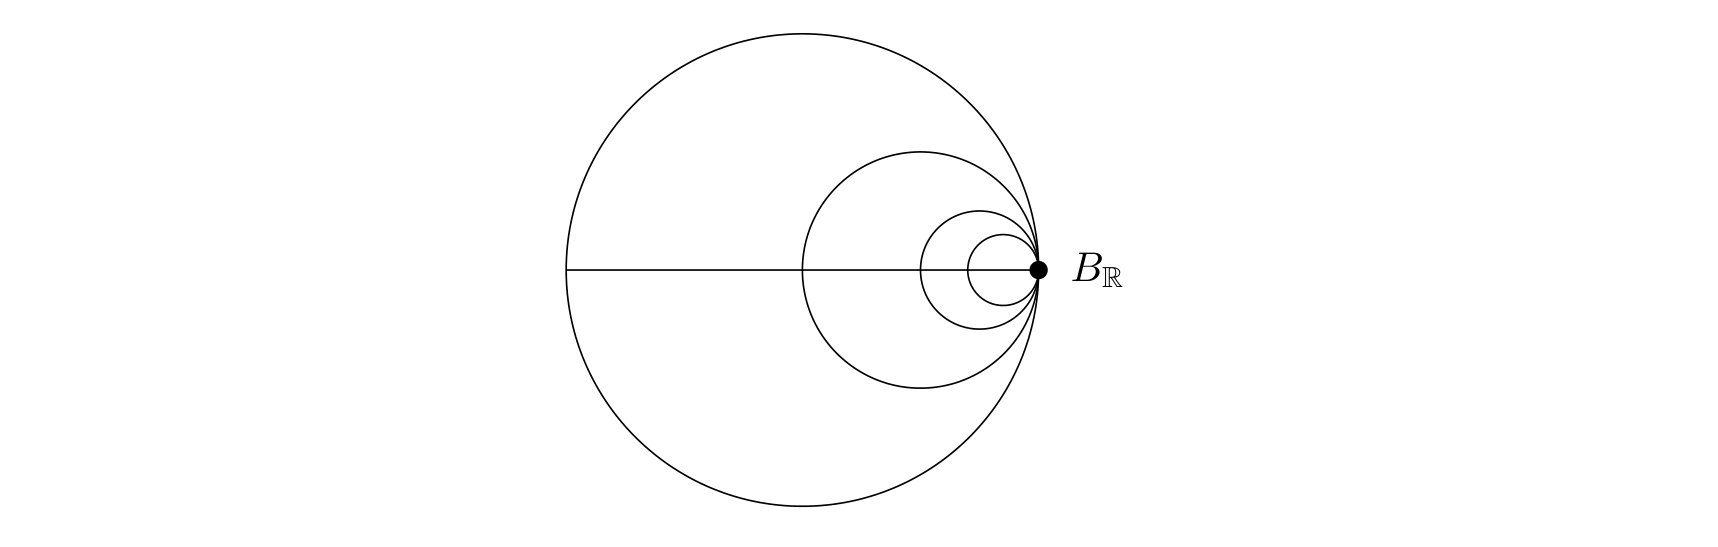
\includegraphics[width=0.42\textwidth]{figure11-3.png}
  \caption{$H=SL_2/SO_2=G_{\R}/K$的 Poincar\'e 圆盘模型。边界上的点对应$B_{\R}$，水平线是一条$T$-轨道，而极限圆（与无穷远点相切的小圆）是$N$-轨道。（原文 p.~198，Figure 11.3）}
  \label{fig:11-3}
\end{figure}

\paragraph{Poincar\'e 圆盘与双曲面模型.}
最熟悉的图景是实版本，即空间$G_{\R}/K$。现在$\R$扮演局部域的角色，因此从复几何的角度看，它与建筑和$\Gr$看起来完全不同。这是双曲空间：
\begin{equation}\tag{11.125}
SL_2(\R)/SO_2\simeq H.
\end{equation}
例如我们可以通过 Poincar\'e 圆盘模型来思考。内部是$G_{\R}/K$，而无穷远点组成$\R\PP^{1}=G_{\R}/B_{\R}$，即$G_{\R}$的旗流形。

现在取一个无穷远点，即一个 Borel $B_{\R}\subset G_{\R}$。对$SL_2$，这是$\R\PP^{1}$中的一个点，即$\R^{2}$中的一条线，而$B_{\R}$是这条线的稳定化子。有一个相应的环面$T$，相应的$T$-轨道是穿过 Poincar\'e 圆盘中心的直线。

现在我们还想画出$N$-轨道。对$SL_2$，
\begin{equation}\tag{11.126}
N=\left\{\begin{pmatrix}1 & b\\ 0 & 1\end{pmatrix}\right\}.
\end{equation}
$N$-作用固定对应于$B_{\R}$的无穷远点，而轨道由图 11.3 中的极限圆（horocycle）给出。

于是我们有$\Gr$的类比——双曲空间$SL_2\R/SO_2$，并且可以映到$SL_2\R/N$，后者称为极限圆空间。然后我们有极限圆对应，它由点$x\in H$连同过它的一条极限圆组成，这个对应空间构成$SL_2(\R)$（模去一个符号）：
\begin{equation}\tag{11.127}
\begin{array}{ccc}
 & SL_2(\R)/(\pm 1) & \\
 \swarrow & & \searrow\\
 SL_2\R/SO_2 & & SL_2\R/N
\end{array}
\end{equation}
极限圆空间实际上可以描述为
\begin{equation}\tag{11.128}
SL_2\R/N\simeq\R^{2}\setminus\{0\}.
\end{equation}

\begin{figure}[htbp]
  \centering
  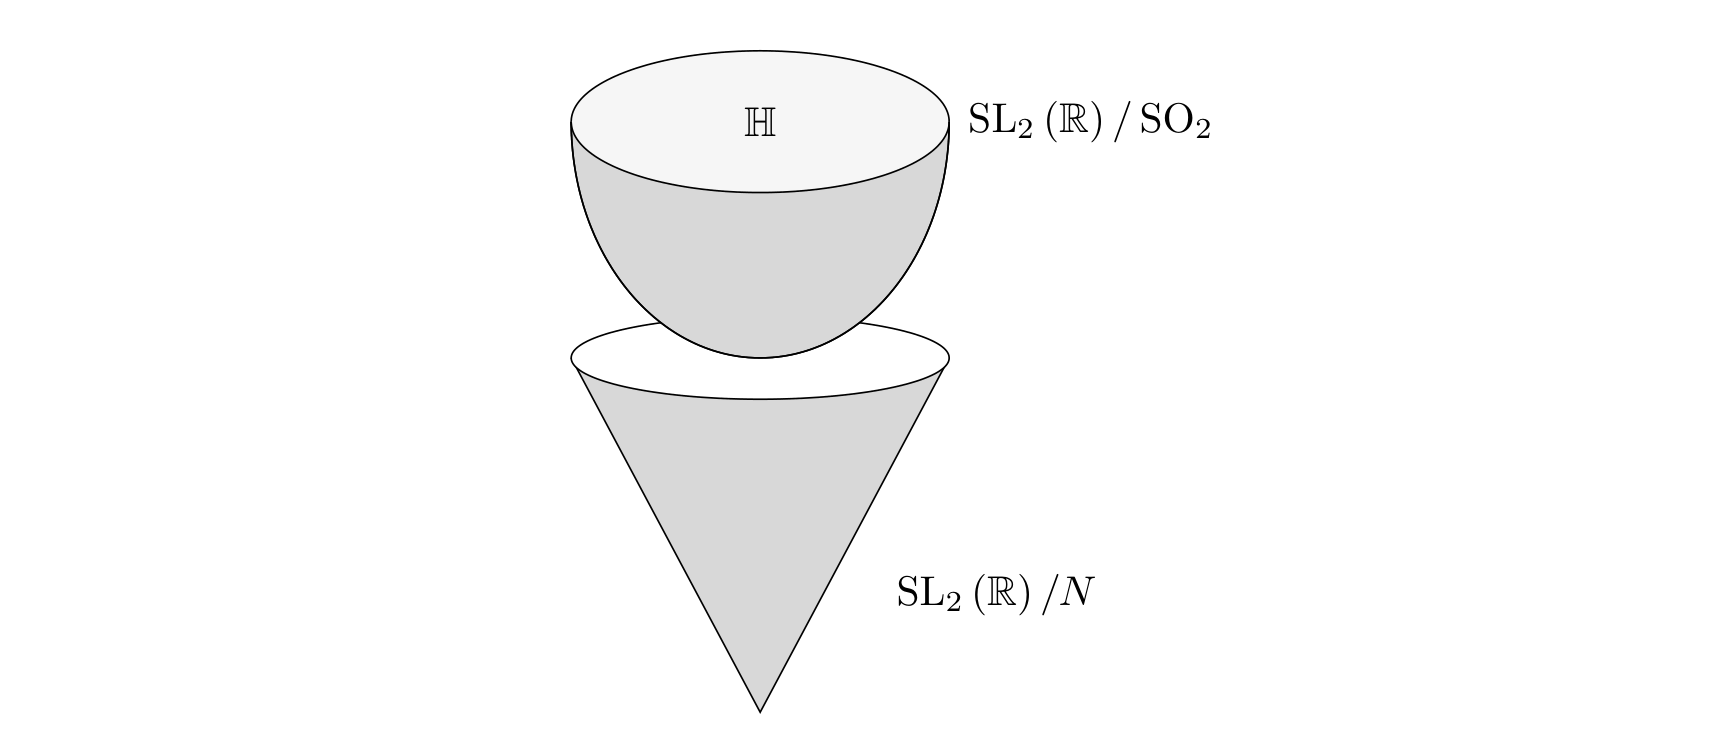
\includegraphics[width=0.42\textwidth]{figure11-4.png}
  \caption{若把$SL_2/SO_2$模型化为双曲面，则可以把极限圆空间$SL_2(\R)/N$看成光锥。（原文 p.~199，Figure 11.4）}
  \label{fig:11-4}
\end{figure}

若把双曲空间模型化为双曲面，这就更容易看出。此时$SL_2\R/N$是$\R^{3}$中的光锥，而$H$作为其中一张叶出现，如图 11.4。在$\infty$附近，$H$看起来像光锥模$\R^{\times}$，即$\R\PP^{1}$。也就是说，我们有一个映射
\begin{equation}\tag{11.129}
\begin{array}{c}
SL_2(\R)/N\simeq\R^{2}\setminus\{0\}\\[2pt]
\downarrow\\[2pt]
\R\PP^{1}=SL_2(\R)/B\\[2pt]
\text{（在 distinguished 点上的纤维为环面 }T\text{）}
\end{array}
\end{equation}
给定$H$上的函数，我们能做的一个自然测量就是沿其中一条极限圆积分。或者我们可以把这看成积分变换。即给定$f\in L^{2}(H)$，我们可以通过 (11.127) 拉回并前推，得到极限圆空间$SL_2(\R)/N$上的函数，即这个光锥上的函数。然后我们可以把它限制到光锥内的任意一条射线上，每条射线对应一个环面$T$。即我们从$H$上的函数出发，拉回、前推、再限制，得到$T$上的函数。现在我们可以用 Fourier 理论分解这个函数。这一程序称为 Harish-Chandra 变换。

为完成与$\Gr_G$的类比，极限圆就是半无限轨道$S_\lambda\subset\Gr$的类比。$\sph$的纤维函子由限制到轨道再前推给出。这里对应的是限制到极限圆再平均（积分）。

还要注意，在图 11.3 中，穿过无穷远不动点的极限圆恰好由$T$-轨道标号。这就是前面“$N(K)$-轨道集合与$\Gr_T$一一对应”这一陈述的类比。

\paragraph{建筑.}
回忆$PSL_2$建筑的顶点是$K^{2}$中的$\cO$-格模去伸缩（即模去位似）。所得的图是图 9.1 和图 9.2 所示的 3-正则树。在无穷远处，这棵树看起来像$\PP^{1}(K)$。极限圆图景的类比如下。

选择一个无穷远点。形式上这意味着树的一个端（end）。这是一个道路的等价类。两条道路若最终在通向无穷远的路上某点重合，即它们只相差有限多个顶点/边，就称等价。

一旦选定了树的一个端，我们就可以考虑距离给定端固定距离的所有顶点的集合。我们说两个顶点$V_1$和$V_2$到该端的距离相同，若存在（在该端的等价类中的）道路$P_1$和$P_2$满足：由于$P_1$和$P_2$在该端的等价类中，它们最终重合，即只相差有限多个顶点；我们要求$P_1$中而不在$P_2$中的边数等于$P_2$中而不在$P_1$中的边数。固定距离的顶点构成一条极限圆。当我们如图 11.5 画出树的公寓（apartment）时，这一点更清楚。这个拉直后的公寓图景是上半空间模型的类比。特定的无穷远点是$i\infty\in H$，而极限圆（$N_{\R}$-轨道）是$H$中的水平线。

\begin{figure}[htbp]
  \centering
  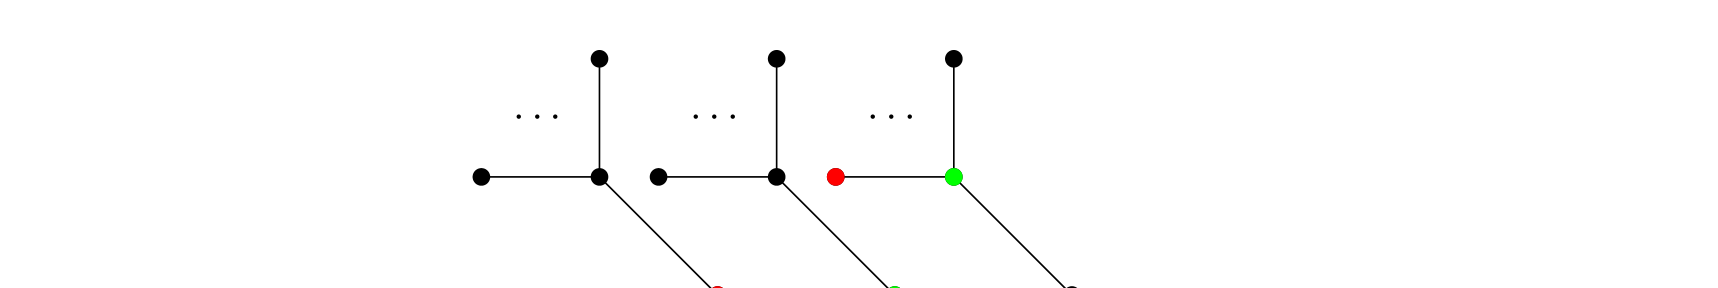
\includegraphics[width=0.5\textwidth]{figure11-5.png}
  \caption{图 9.2 中 3-正则树的公寓。绿色顶点彼此到该端的距离相同，红色顶点到该端的距离也相同。（原文 p.~200，Figure 11.5）}
  \label{fig:11-5}
\end{figure}

% [Tutor Note: (11.125) 中的$H$是双曲平面；$G_{\R}/K$与$\Gr_G$的类比并非同构，而是“非紧对称空间 vs. 仿射 Grassmann 流形”的层次类比。这里$N_{\R}$-轨道（极限圆）对应$N(K)$-轨道（半无限轨道$S_\lambda$），而$T$-轨道对应不动点格$\Gr_T\simeq\Lambda$；Mirkovi\'c–Vilonen 的纤维函子正是“沿极限圆积分”的代数版本。]

\section{谱分解}\label{sec:11-7}

\begin{sectionkey}
本节把$\sph\simeq\Rep(G^{\vee})$的作用推广到曲线上的每一点，得到$\otimes'_{x\in C}\Rep(G^{\vee})$在$\Shv(\Bun_G(C))$上的作用，并猜想它分解到 \term{Langlands 参数空间}{space of Langlands parameters} $\Loc_{G^{\vee}}(C)$上；谱纤维的对象即 Hecke 特征层，对应调和分析中的特殊函数。
\end{sectionkey}

\begin{flushright}\small 第 29 讲；2021 年 5 月 20 日\end{flushright}

\subsection{Langlands 对偶群}\label{sec:11-7-1}

回忆我们把几何 Satake 对应看作描述理论$A_G$的线算子$\otimes$-范畴：
\begin{equation}\tag{11.130}
\sph:=A_G(S^{2})=\Shv(LG_+\backslash LG/LG_+).
\end{equation}
它以 Hecke 修正作用在$\Shv(\Bun_G(C))$上。然后几何 Satake 的结果是
\begin{equation}\tag{11.131}
(\sph,*)\simeq\Rep(G^{\vee}),
\end{equation}
其中$G^{\vee}$是 Langlands 对偶群。这是$k$上的约化代数群（$k$是我们的层的系数域）。

这个群$G^{\vee}$有一些粗特征，例如
\begin{equation}\tag{11.132}
\pi_1(G)\simeq Z(G^{\vee})^{\vee}.
\end{equation}
所以若$G$单连通，则$G^{\vee}$是伴随型（无中心）。对极大环面$T\subset G$，对偶环面$T^{\vee}$是$G^{\vee}$的极大环面。事实上，$G^{\vee}$的构造自带对偶环面，所以$G^{\vee}$真正是一个分裂约化群。

\begin{srcrem}{82}
$G^{\vee}$实际上自带一个 pinning。所以它带有环面$T^{\vee}\subset G^{\vee}$，但也带有一个典范余特征
\begin{equation}\tag{11.133}
G_m\subset T^{\vee}\subset G^{\vee},
\end{equation}
我们将称之为$2\rho^{\vee}$。这个包含对应于纤维函子
\begin{equation}\tag{11.134}
\Vect^{\Z\text{-gr}}\leftarrow\Vect^{\Lambda\text{-gr}}\leftarrow\Rep G^{\vee}.
\end{equation}
要点是：纤维函子$\sph\to\Vect$分解为上同调到分次向量空间的函子与$\operatorname{Forget}$：
\begin{equation}\tag{11.135}
\Vect\xleftarrow{\ \operatorname{Forget}\ }\Vect^{\Z\text{-gr}}\xleftarrow{\ H^{*}\ }\sph.
\end{equation}
\end{srcrem}
特别地，这个典范的$G_m\subset T^{\vee}$给出表示的典范分次，这为我们挑出一个 Borel（所有正的东西）。

\begin{srcex}{78}
从环面$T$出发，Langlands 对偶就是对偶环面$T^{\vee}$。$GL_n$的 Langlands 对偶是它自己：
\begin{equation}\tag{11.136}
GL_n^{\vee}=GL_n.
\end{equation}
Langlands 对偶交换伴随型和单连通群，例如
\begin{equation}\tag{11.137}
PGL_n^{\vee}=SL_n.
\end{equation}
$D_n$型自对偶：
\begin{equation}\tag{11.138}
SO_{2n}^{\vee}=SO_{2n}.
\end{equation}
另一方面，$B_n$型与$C_n$型互换：
\begin{equation}\tag{11.139}
SO_{2n+1}^{\vee}=Sp_{2n}.
\end{equation}
\end{srcex}
这是要记住的：群$SO_{2n+1}$与$Sp_{2n}$看起来并无关系（例如它们的几何非常不同），但它们的组合数据是对偶的。这就是为什么涉及 Langlands 对偶的东西往往非常深刻：所涉及的群往往（以显然的方式）互不相关。

\subsection{本征对象}\label{sec:11-7-2}

回忆我们引入这个范畴来作用于事物。设$C$是黎曼面/代数曲线。则对$x\in C$我们得到一个作用：$\sph\circlearrowright\Shv(\Bun_G(C))$。具体地，$V\in\sph$定义$\operatorname{Hecke}_x$上的层，它通过对应
\begin{equation}\tag{11.140}
\begin{array}{ccc}
 & \operatorname{Hecke}_x & \\
 \swarrow & & \searrow\\
 \Bun_G & & \Bun_G
\end{array}
\end{equation}
给出从$\Bun_G$上的层到自身的积分变换。回忆我们在例 70 和 71 中对$G=GL_n$见过这一点。所以我们有一个交换$\otimes$-范畴$\sph\simeq\Rep(G^{*})$在范畴$\Shv(\Bun_G)$上的作用，并想作谱分解。于是我们要识别\term{本征对象}{eigenobject}，即我们只是试图同时对角化一堆算子。

本征对象是一个对象$F\in\Shv(\Bun_G)$连同一个同构
\begin{equation}\tag{11.141}
V*F\xrightarrow{\ \sim\ }E_x(V)\otimes F
\end{equation}
对$V\in\Rep(G^{\vee})\simeq\sph$。即$E_x(-)$是“本征值”。这是一个函子
\begin{equation}\tag{11.142}
E_x\colon\Rep(G^{\vee})\xrightarrow{\ \otimes\ }\Vect.
\end{equation}
用我们的 Tannakian 故事，我们可以容易地写下本征值。要点是$\Rep(G^{\vee})=\Shv(\mathrm{pt}/G^{\vee})$而$\Vect=\Shv(\mathrm{pt})$，所以这样的函子等价于一个映射$\mathrm{pt}\to\mathrm{pt}/G^{\vee}$。但这样的映射在相差同构的意义下只有一个。等价地，这样的映射由一个$G^{\vee}$-torsor $E_x$给出。然后给定$V\in\Rep(G^{\vee})$，我们可以把它送到伴随向量丛：$(V)_{E_x}\in\Vect$。

现在我们可以做两件事：变化点，或去范畴化（取某些迹）。首先我们变化点。

% [Tutor Note: (11.142) 中“$\otimes$标记的箭头”表示这是张量函子（$\otimes$-functor）；$E_x$之所以由$G^{\vee}$-torsor 给出，是因为 Tannakian 对偶把$\Shv(\mathrm{pt})$上的张量函子等同于$\mathrm{pt}/G^{\vee}$的一个点（即$G^{\vee}$-torsor）。原文把$G^{\vee}$的法向分次（由$2\rho^{\vee}$给出）单独列出，是为了让“本征值”与表示的分次相容。]

\subsection{变化点}\label{sec:11-7-3}

现在我们变化点$x\in C$。于是不再由单个$\Rep(G^{\vee})$拷贝作用，而是将由$C$的某个点集上每个点处的一个这样的范畴作用。

更形式地，我们有一个受限张量积\footnote{这与之前受限积类似定义：除有限多个“条目”外均为平凡。}的作用：
\begin{equation}\tag{11.143}
\bigotimes'_{x\in C}\Rep(G^{\vee})\circlearrowright\Shv(\Bun_G(C)).
\end{equation}
即我们在一大堆点处作修正，而不只是在一个点。

我们一直有一个基本假设：周围有一个拓扑场论。即我们受到$A_G(C)=\Shv(\Bun_G(C))$这一想法的驱动，而上面的作用应由线算子范畴给出。它来自 TFT 这一事实意味着线算子的作用局部地、常数地依赖于$x\in C$。于是这个作用通过$R_C\Rep(G^{\vee})$的作用分解：
\begin{equation}\tag{11.144}
\begin{array}{ccc}
\bigotimes'_{x\in C}\Rep(G^{\vee}) & \longrightarrow & \Shv(\Bun_G(C))\\
 & \searrow & \nearrow\\
 & & R_C\Rep(G^{\vee})
\end{array}
\end{equation}
事实上我们说过：
\begin{align}
\Spec\int_C\Rep(G^{\vee})&=\operatorname{Map}_{lc}(C,\mathrm{pt}/G^{\vee})\tag{11.145}\\
&=\Loc_{G^{\vee}}(C).\tag{11.146}
\end{align}

\begin{srcrem}{83}
$\Loc_{G^{\vee}}(C)$在拓扑/Betti 情形下极其简单。具体地，它是
\begin{align}
\Loc_{G^{\vee}}(C)&=\{\pi_1(C)\to G^{\vee}\}/G^{\vee}\tag{11.147}\\
&=\Bigl\{A_1,\dots,A_g,B_1,\dots,B_g\in G^{\vee}\ \Big|\ \prod_i A_iB_iA_i^{-1}B_i^{-1}=1\Bigr\}/G^{\vee},\tag{11.148}
\end{align}
因为黎曼面的基本群有$A$、$B$圈的这种简单呈现。
\end{srcrem}

这一认识的结果是，如果我们相信它来自一个场论：
\begin{equation}\tag{11.149}
A_G(C)=\Shv(\Bun_G(C)),
\end{equation}
那么$\bigotimes'\Rep G^{\vee}$在其上的作用分解为
\begin{equation}\tag{11.150}
\begin{array}{ccc}
\bigotimes'_{x\in C}\Rep(G^{\vee}) & \longrightarrow & \Shv(\Bun_G(C))\\
 & \searrow & \nearrow\\
 & & \QC(\Loc_{G^{\vee}}(C))
\end{array}
\end{equation}
事实上，沿着这些思路有一些（非常深刻且困难的）定理，适用于各种版本的$\Shv$。

\begin{srcthm}{10（Gaitsgory 消没定理）}
这在 de Rham 情形成立。即朴素的 Hecke 作用
$\QC(\Loc^{dR}_{G^{\vee}})\circlearrowright D(\Bun_G(C))$通过相应的整体对象分解。
\end{srcthm}

\begin{srcthm}{11（Nadler–Yun）}
这在 Betti 情形成立，其中我们的层具有幂零奇异支撑：$\Shv_N(\Bun_G(C))$。
\end{srcthm}

\begin{srcrem}{84}
$\Shv_N(\Bun_G(C))$是我们从$\Bun_T$、$\Bun_L$（$L$为 Levi 子群）上的局部常值层出发并诱导得到的范畴。
\end{srcrem}

\begin{srcthm}{12（Arinkin–Gaitsgory–Kazhdan–Raskin–Rozenblyum–Varshavsky）}
这在受限情形（在$\F_q$上）成立。\footnote{这算是 de Rham 世界与 Betti 世界的交叠，即某种“核心”的几何 Langlands。}
\end{srcthm}

这告诉我们$\Shv(\Bun_G(C))$在$\Loc_{G^{\vee}}$（Langlands 参数空间）上谱分解。即$A_G(C)$是$\Loc_{G^{\vee}}$上的范畴层。这是 Langlands 对应的要点之一。

我们能问的最具体的东西是某点$E\in\Loc_{G^{\vee}}$处的纤维。这将是$E$-Hecke \term{特征层}{eigensheaf}的集合。这是一个层$F\in\Shv(\Bun_G)$连同同构
\begin{equation}\tag{11.151}
V_x*F\xrightarrow{\ \sim\ }(V_x)_{E_x}\otimes F
\end{equation}
对所有$x\in C$和$V\in\Rep(G^{\vee})$成立。即$F$是曲线上每一点处 Hecke 算子的本征对象，本征值是$E\in\Loc_{G^{\vee}}$，即我们在每点有本征值（$G^{\vee}$-torsors），并把它们拼成局部常值层$E$。

这些是调和分析中特殊函数概念在范畴层面的类比。特殊函数往往满足非常好的微分方程组。特别地，交换微分算子族的本征函数就是特殊函数，例如指数函数$e^{\lambda x}$。所以 Hecke 特征层是$e^{\lambda x}$的类比，其中本征值$\lambda$现在被曲线$C$上的$G^{\vee}$-局部系统$E$取代。

我们在交换情形谈过 Hecke 特征层，那时可以用例如 Abel–Jacobi 映射或 Fourier–Mukai 变换来构造它们。但在非交换情形没有容易的构造方法。对任何特定的局部系统，都不清楚是否存在。但这仍把我们引向朴素的几何 Langlands 猜想。

% [Tutor Note: 11.7.2 开头原文把右端误写作$\Rep(G^{*})$（星号），其后一律为$G^{\vee}$；译文保留该处笔误形式以对应原文，读者应读作$G^{\vee}$。(11.145) 的$\operatorname{Map}_{lc}$指局部常值映射，其叠结构使$\Spec$只能取导出意义；原文在 Betti 情形下不加导出修饰，读者需自行补上。]

\section{朴素的几何 Langlands 猜想}\label{sec:11-8}

\begin{sectionkey}
本节陈述朴素猜想$A_G(C)\simeq\QC(\Loc_{G^{\vee}})$，指出它因$\Loc_{G^{\vee}}$的奇点而失败，并说明修正方向：限制到不可约局部系统（对应$B$-侧的尖点层）或改用导出/幂零支撑版本；最后把几何 Satake 解释为$A_G$与 4 维 B-模型之间的线算子匹配。
\end{sectionkey}

朴素的几何 Langlands 猜想大致是说：存在足够多的 Hecke 特征层，且它们张成整个范畴。也就是说
\begin{equation}\tag{11.152}
A_G(C)\simeq\QC(\Loc_{G^{\vee}}),
\end{equation}
其中摩天楼层$\cO_E\in\QC(\Loc_{G^{\vee}})$对应于一个 Hecke 特征层$A_E\in A_G(C)$，后者在相差一个标量的意义下唯一。

\begin{srcrem}{85}
这类似于低一层的图景：指数函数张成$L^{2}$意味着我们有 Fourier 变换。
\end{srcrem}

于是对每个$E\in\Loc_{G^{\vee}}$我们得到$A_E\in A_G(C)$，在相差标量意义下唯一。等价地说，这是在说
\begin{equation}\tag{11.153}
\QC(\Loc_{G^{\vee}})\circlearrowright\Shv(\Bun_G)
\end{equation}
是自由秩$1$模。换言之，这个模由本征向量张成。更具体地，我们可以选一个合适的循环向量让它作用，例如 Whittaker 层，于是这是说诱导出的态射是等价：
\begin{equation}\tag{11.154}
\QC(\Loc_{G^{\vee}})\xrightarrow{\ \sim\ }\Shv(\Bun_G).
\end{equation}
这是 Fourier 理论中单位元处摩天楼层的类比。

这个猜想按原样并不成立，这一点早已为人所知。基本问题在于叠$\Loc_{G^{\vee}}$是奇异的，而$\QC(\Loc_{G^{\vee}})$检测不到这些奇点。所以我们可以苦思并修正它，或者限制到$\Loc_{G^{\vee}}$内一个由不可约局部系统组成的开稠密轨迹。对$G=GL_n$，这恰指不可约的带平坦联络向量丛（即没有在平行移动下封闭的子丛）。一般而言，一个局部系统不可约，若它没有平坦的到抛物子群的约化。于是我们有由不可约局部系统组成的开稠密轨迹$\Loc^{irr}_{G^{\vee}}$。结果这是一个光滑叠，几乎是一个簇。若$E$不可约，则
\begin{equation}\tag{11.155}
\Aut(E)=Z(G^{\vee}).
\end{equation}
例如若$G$单连通，则$G^{\vee}$伴随，故这些自同构是平凡的。所以此时$\Loc^{irr}_{G^{\vee}}$构成一个光滑簇。

无论如何，猜想预期在这个轨迹上成立。$G=SL_2$的情形归功于 Drinfeld，$G=GL_n$的情形归功于 Gaitsgory。（原文此处附引用标记。）

限制到不可约局部系统在另一侧对应什么？不可约局部系统意味着没有到抛物子群$P^{\vee}\subset G^{\vee}$的约化，这等价于不在任何映射的像中：$\Loc_{P^{\vee}}\to\Loc_{G^{\vee}}$。特别地，它与这些抛物诱导/Eisenstein 级数对应没有交互：
\begin{equation}\tag{11.156}
\begin{array}{ccc}
 & \Loc_{P^{\vee}} & \\
 \swarrow & & \searrow\\
 \Loc_{G^{\vee}} & & \Loc_{G^{\vee}}
\end{array}
\end{equation}
即它与 Eisenstein 级数没有交互。

在 Langlands 对应的另一侧，这意味着我们在找$F\in\Shv(\Bun_G)$使得抛物限制
\begin{equation}\tag{11.157}
\begin{array}{ccc}
 & \Bun_P & \\
 \swarrow & & \searrow\\
 \Bun_G & & \Bun_L
\end{array}
\end{equation}
为零。这就是\term{尖点}{cuspidal}的定义。

\begin{srcex}{79}
尖形式（cusp form）是在$\infty$处为$0$的模形式。结果这等价于常数项为$0$。回忆常数项由沿一条水平线/极限圆积分给出，而这个操作恰好是从$PSL_2\to T$的抛物限制。
\end{srcex}
所以$B$-侧尖点的层应当与$A$-侧不可约轨迹上的层相匹配。

\paragraph{为什么它不能成立.}
朴素的几何 Langlands 猜想失败，原因如下。对应于
\begin{equation}\tag{11.158}
E=\mathrm{triv}\in\Loc_{G^{\vee}}(C)
\end{equation}
的$\Bun_G$上的“那个”自守层是什么？平凡局部系统是最糟糕的点。它是最奇异/最像栈（自同构最多）的点。看出这令人困惑的一种方式是：$\mathrm{triv}$来自$\mathrm{triv}_{T^{\vee}}$。但它也来自任何 Levi $L$的$\mathrm{triv}_{L^{\vee}\subset G^{\vee}}$。而 Eisenstein 级数理论给我们一个公式：
\begin{equation}\tag{11.159}
A_{\mathrm{triv},L^{\vee}}\in\Shv(\Bun_G),
\end{equation}
通过做某种版本的抛物诱导，而它们全都不同。所以我们有一堆层，它们都想以平凡局部系统作为本征值。

另一个密切相关的事情是尝试$\Bun_G$上最显然的层，即常值层$k$。它是 Hecke 特征层吗？当我们在$x$处作用 Hecke 算子$V_x$于$k$上时，得到$V_x*k$，它是$k$的拉回限制到某个$G(\cO)$-轨道（或更一般地，把它与$\Gr$上某个层作张量）后的前推。所以结果是层$H_V\in\Shv(\Gr)$的上同调与$k$张量。于是对任意点$x\in C$我们得到同样的东西：$k$与这个上同调张量，它可能生活在非零次数。这称为 Arthur 特征层。这些正是我们缺失的那类东西。

\subsection{朴素的电磁/Montonen–Olive $S$-对偶}\label{sec:11-8-1}

一旦我们对朴素几何 Langlands 猜想感觉良好，就可以放开手脚，作朴素的猜测：整个理论$A_G$等价于$B^{\mathrm{naive}}_{G^{\vee}}$，即$\mathrm{pt}/G^{\vee}$上的 4 维 B-模型（回忆第 10.7 节）。回忆它给出：
\begin{align}
B^{\mathrm{naive}}_{G^{\vee}}(M^{3})&=\cO(\Loc_{G^{\vee}}(M))\tag{11.160}\\
B^{\mathrm{naive}}_{G^{\vee}}(\Sigma^{2})&=\QC(\Loc_{G^{\vee}}(\Sigma))\tag{11.161}\\
B^{\mathrm{naive}}_{G^{\vee}}(N^{1})&=\Shv\mathrm{Cat}(\Loc_{G^{\vee}}(N)).\tag{11.162}
\end{align}
与其说这是猜想的“朴素”版本，不如说这是第一近似。回忆我们是用线算子范畴构造$G^{\vee}$（从而构造$B^{\mathrm{naive}}_{G^{\vee}}$）的。我们本可以从局部算子出发得到第零近似，但在这个（非导出的）情形下那会是平凡的。这个理论可能不包含匹配理论$A_G$所需的全部信息，但它们几乎相同。

若$A_G$与$B_{G^{\vee}}$作为场论等价，这当然意味着线算子及其作用必须一致。在$A$-侧我们有$A_G(S^{2})=\sph$，而在$B$-侧我们有
\begin{equation}\tag{11.163}
B_{G^{\vee}}(S^{2})=\QC\bigl(\Loc_{G^{\vee}}(S^{2})\bigr).
\end{equation}
由于$S^{2}$单连通，$\Loc_{G^{\vee}}(S^{2})\simeq\mathrm{pt}/G^{\vee}$，所以至多差一些导出增强，我们得到
\begin{equation}\tag{11.164}
\QC\bigl(\Loc_{G^{\vee}}(S^{2})\bigr)=\QC(\mathrm{pt}/G^{\vee}).
\end{equation}
即便我们（导出地）正确地说这件事，仍然有
\begin{equation}\tag{11.165}
\Rep(G^{\vee})\subset\QC\bigl(\Loc_{G^{\vee}}(S^{2})\bigr).
\end{equation}
这些是 Wilson 线算子。我们可以如下显式地看出这个作用。设$C$是黎曼面，$x\in C$，$V\in\Rep(G^{\vee})$。则我们如下得到$\Loc_{G^{\vee}}(C)$上的向量丛。对任何局部系统，我们可以考虑$V$的伴随向量丛，并取它在$x$处的纤维：
\begin{equation}\tag{11.166}
E\mapsto(V)_{E_x}.
\end{equation}
也就是说，有一个由拉回给出的函子
\begin{equation}\tag{11.167}
\Rep(G^{\vee})\xrightarrow{\ i_x^{*}\ }\QC(\Loc_{G^{\vee}}),
\end{equation}
其中
\begin{equation}\tag{11.168}
i_x\colon\Loc_{G^{\vee}}\to\mathrm{pt}/G^{\vee}
\end{equation}
取$x$处的纤维。换言之，给定$x\in C$和$V\in\Rep(G^{\vee})$有一个算子
\begin{equation}\tag{11.169}
V*(-)\colon\QC(\Loc_{G^{\vee}})\to\QC(\Loc_{G^{\vee}}).
\end{equation}
这些就是 Wilson 线算子。

于是朴素等价$A_G$与$B^{\mathrm{naive}}_{G^{\vee}}$蕴含线算子在两侧必须匹配：
\begin{equation}\tag{11.170}
A_G(S^{2})\simeq B_{G^{\vee}}(S^{2}).
\end{equation}
这个陈述就是几何 Satake。在谱/$B$-侧，线算子就是这些非常简单的 Wilson 线；而在自守/$A$-侧我们有的是更复杂的 't Hooft 线。然后几何 Satake 告诉我们它们相同。

接着朴素几何 Langlands 猜想说我们有一个范畴等价，并且对每个点$x\in C$有相容的作用：
\begin{equation}\tag{11.171}
\begin{array}{ccc}
\Shv(\Bun_G) & \xrightarrow{\ \simeq\ } & \QC(\Loc_{G^{\vee}})\\
\uparrow & & \uparrow\\
\sph & \xrightarrow{\ \simeq\ } & \Rep(G^{\vee})
\end{array}
\end{equation}

\begin{flushright}\small 第 30 讲；2021 年 5 月 27 日\end{flushright}

% [Tutor Note: (11.152) 按原样不成立，正确的修正通常是把$\QC$换成$\IndCoh$（Arinkin–Gaitsgory 的“修正几何 Langlands 猜想”），因为$\Loc_{G^{\vee}}$奇异时$\QC$丢失了导出信息；这也是 (11.165) 只能是包含而非等号的原因。(11.159) 中的$A_{\mathrm{triv},L^{\vee}}$依赖 Levi $L$，不同$L$给出不同的 Eisenstein 层，但都以平凡局部系统为本征值——这正是“本征值不能唯一确定本征对象”的表现。]

